\documentclass[10pt]{article}

%% Packages
\usepackage[margin=1in, top=0.75in]{geometry}
\usepackage[utf8]{inputenc}
\usepackage[T1]{fontenc}
\usepackage[usenames,dvipsnames]{xcolor}
\usepackage{amssymb, amsfonts, amsmath, mathrsfs, enumitem, tcolorbox, bbm, graphicx, fullpage, parskip, mathtools, float, amsthm}
\usepackage{tikz,sgame,bbm,todonotes, setspace, soul}
\usepackage[english]{babel}

\setcounter{tocdepth}{2}
% Links (and references)
\definecolor{linkblue}{RGB}{40, 50, 200}
\usepackage[colorlinks=true, allcolors={linkblue}]{hyperref}

%% Math operators
\newcommand*{\ones}{\text{\usefont{U}{bbold}{m}{n}1}}
\newcommand{\reals}{\mathbb{R}}
\newcommand{\rationals}{\mathbb{Q}}
\newcommand{\integers}{\mathbb{Z}}
\newcommand{\naturals}{\mathbb{N}}
\newcommand{\complex}{\mathbb{C}}
\newcommand{\normal}{\mathcal{N}}

% General math
\newcommand{\abs}[1]{\mathop{\left|#1\right|}} % absolute value
\newcommand{\inv}{^{-1}} % inverse
\let\oldST\st
\newcommand{\strikethrough}{\oldST}
\renewcommand{\st}{\;\text{s.t.}\;} % math operator for "such that"
\newcommand{\eg}{\emph{e.g.} }
\newcommand{\ie}{\emph{i.e.} }
\newcommand{\interior}{\mathop{\rm int}}

% Optimization
\newcommand{\argmax}{\mathop{\rm argmax}}
\newcommand{\argmin}{\mathop{\rm argmin}}
\newcommand{\opt}{^\star}
% Analysis, vector spaces, and topology
\newcommand{\set}[1]{\left\{#1\right\}} % set notation
\newcommand{\seq}[1]{_{#1}^{\infty}} % add sequence notiation to set (or to a summation symbol for series)
\newcommand{\setless}{\mathop{\backslash}} % A \ B notation
\newcommand{\pow}{\mathop{\mathcal{P}}} % power set
\newcommand{\im}{\mathop{\rm im}} % image
\newcommand{\spans}{\mathop{\rm span}} % span
\newcommand{\rank}{\mathop{\rm rank}} % rank
\newcommand{\topo}{\mathop{\mathcal{T}}} % topology
\newcommand{\cont}{\mathop{\bf C}} % continuously differentiable

% Matrices
\newcommand\colvector[1]{\begin{bmatrix}#1\end{bmatrix}}
\newcommand\rowvector[1]{\begin{bmatrix}#1\end{bmatrix}}
\newcommand\matrixc[1]{\begin{bmatrix}#1\end{bmatrix}}
\newcommand\matrixp[1]{\begin{pmatrix}#1\end{pmatrix}}
\newcommand\detmatrix[1]{\begin{vmatrix}#1\end{vmatrix}}
\newcommand\rankmatrix{\begin{bmatrix}I_r & \rvline & \mathbf{0}_1\\\hline \mathbf{0}_2 & \rvline & \mathbf{0}_3 \end{bmatrix}}

% Statistics
\newcommand{\cov}{\mathop{\rm cov}} % covariance
\newcommand{\corr}{\mathop{\rm corr}} % correlation
\newcommand{\expect}{\mathop{\mathbb{E}}} % expectation
\newcommand{\indep}{\perp \hspace{-1.4ex} \perp} % independence symbol
\newcommand{\distiid}{\mathop{\overset{\text{i.i.d.}}\sim}} % i.i.d.
\newcommand{\oversim}[1]{\mathop{\overset{\text{#1}}\sim}} % general text over \sim
\newcommand{\prob}{\mathbb{P}}
\newcommand{\mse}{\mathop{\rm MSE}}
\newcommand{\var}{\mathop{\rm Var}}
\newcommand{\sd}{\mathop{\rm sd}}
\newcommand{\se}{\mathop{\rm se}}
\newcommand{\bias}{\mathop{\rm bias}}
\newcommand{\toprob}{\overset{p}{\to}}
\newcommand{\toas}{\overset{a.s.}{\to}}
\newcommand{\todist}{\overset{d}{\to}}
\newcommand{\hyp}{\mathbb{H}}

% Economics
\newcommand{\choice}{\mathop{C_{\succsim}}} % choice correspondence

% Update existing operators
\let\oldExists\exists
\renewcommand{\exists}{\oldExists\;}
\let\oldForall\forall
\renewcommand{\forall}{\;\oldForall\;}
\let\oldEmptyset\emptyset
\renewcommand{\emptyset}{\mathop{\varnothing}}
\newcommand{\parl}{\left(}
\newcommand{\parr}{\right)}
\newcommand{\midbar}{\middle|}
\newcommand{\barl}{\left[}
\newcommand{\barr}{\right]}
\newcommand{\curll}{\left\{}
\newcommand{\curlr}{\right\}}


%% Presentation environments
% Proofs, counterexamples, and disproofs
\renewcommand\qedsymbol{$\openbox$}
\renewenvironment{proof}{{\raggedright \textit{\textbf{Proof.}}}}{\qed} % Proof
\newenvironment{pf}{\begin{proof}}{\end{proof}} % Proof (shorthand)

\newenvironment{disproof}{{\raggedright \textit{\textbf{Disproof.}}}}{$\qed$} % Disproof
\newenvironment{counterex}{{\raggedright \textit{\textbf{Counterexample.}}}}{} % Counterexample

% Theorem styles
\theoremstyle{plain}
\newtheorem{result}{Result}
\newtheorem{lemma}{Lemma}[section]
\newtheorem{assumption}{Assumption}[section]
\newtheorem{theorem}{Theorem}[section]
\newtheorem{proposition}{Proposition}[section]
\newtheorem{corollary}{Corollary}[section]
\newtheorem{axiom}{Axiom}[section]
\theoremstyle{definition}
\newtheorem*{example}{Example}
\newtheorem*{definition}{Definition}
\newtheorem*{exercise}{Exercise}
\newtheorem*{model}{Model}
\newtheorem*{proposition*}{Proposition}
\newtheorem*{model*}{Model}
\newtheorem*{solution}{Solution}
\newtheorem*{remark}{Remark}
\newtheorem*{question}{Question}
\newtheorem*{answer}{Answer}
\newtheorem*{algorithm}{Algorithm}

\newcommand{\blue}[1]{\textcolor{blue}{\emph{#1}}}
\newcommand{\red}[1]{\textcolor{red}{\emph{#1}}}




\newcommand{\gabe}[1]{\todo[inline,color=green!20!white]{\textbf{GS:} #1}}


%% Header
\makeatletter
\newcommand{\course}[1]{\def\@course{#1}}
\newcommand{\term}[1]{\def\@term{#1}}
\renewcommand{\title}[1]{\def\@entitle{#1}}
\renewcommand{\maketitle}{
    \begin{tcolorbox}[colframe=darkgray]
        \begin{center}
            \textbf{\@course} \\[0.25em]
            {\Large\textit{\@entitle}} \\[0.5em]
            Gabe Sekeres \\[0.5em]
            \@term
        \end{center}
    \end{tcolorbox}
    \vspace{1em}
}
\makeatother


%% Code
\usepackage{listings}
\usepackage{beramono}
\lstdefinelanguage{Julia}%
  {morekeywords={abstract,break,case,catch,const,continue,do,else,elseif,%
      end,export,false,for,function,immutable,import,importall,if,in,%
      macro,module,otherwise,quote,return,switch,true,try,type,typealias,%
      using,while},%
   sensitive=true,%
   alsoother={$},%
   morecomment=[l]\#,%
   morecomment=[n]{\#=}{=\#},%
   morestring=[s]{"}{"},%
   morestring=[m]{'}{'},%
   breaklines=true,%
}[keywords,comments,strings]%

\lstset{%
    language         = Julia,
    basicstyle       = \ttfamily,
    keywordstyle     = \bfseries\color{blue},
    stringstyle      = \color{magenta},
    commentstyle     = \color{ForestGreen},
    showstringspaces = false,
}






\title{Econometrics I: Chen Qiu}
\author{Gabe Sekeres}
\course{ECON 6190}
\term{Fall 2024}
\begin{document}
\maketitle

\tableofcontents

\newpage

\paragraph{Class Information} This is a really exciting time to learn Econometrics, especially at Cornell. There's a long history at Cornell of treating Econometrics essentially as a decision problem. For Chen, Econometrics is useful and powerful because it helps people make decisions with their data.

The course material will be divided into three parts:
\begin{enumerate}
	\item Introduction to statistical inference
	\item Large-sample approaches to statistical inference
	\item Classical theory of estimation and inference
\end{enumerate}

There will be in-class midterms on Tuesday Octover 8 and Tuesday November 5.

\section{Introduction to Statistical Inference}

\subsection{Sampling Models}

Economists often collect data that consist of some observations on variables of interest. Statistically, this is a random sample from a large population, from which we can learn about the population.

We call $X$ a random variable / vector of interest (\eg, wage and education in the US). We say that $X \sim F$ where $F$ is the true distribution of wage and education in the US. $X = (X_w,X_e)$. We might be interested in the joint CDF of $X$, denoted $F(x_w,x_e) = P\{X_w \le x_w,\; X_e \le x_e\}$. We could extend these notions to the discrete case, where there is a joint PMF, $f(x_w,x_e) = P\{X_w = x_w,\;X_e = x_e\}$. We can also define the joint PDF in the continuous case, 
\[
f(x_w,x_e) = \frac{\partial^2 F(x_w,x_e)}{\partial x_w \partial x_e}
\]
and note that $\int_{-\infty}^\infty\int_{-\infty}^\infty f(u,w) dudw = 1$. Therefore, we have that
\[
F(x_w,x_e) = P\{X_w \le x_w,\; X_e \le x_e\} = \int_{-\infty}^{x_w} \int_{-\infty}^{x_e} f(u,w) dw du
\]

We may also be interested in the \blue{marginal distribution}, which says that given some $\{X_w,X_e\}$, we might be interested in the distribution of the wage ($X_w$) irrespective of the education ($X_e$). We say that the marginal distribution (or marginal CDF) is
\[
F_{X_w}(x_w) = P\{X_w \le x_w\} = P\{X_w \le x_w,\; X_e \le \infty\}
\]
In the continuous case, we have the (marginal) pdf of $X_W$ which is $f_{X_w}(x_w)= \int_{-\infty}^\infty f(x_w,x_e) dx_e$.

In the discrete case, the (marginal) pmf of $X_W$ is $f_{X_w}(x_w) = P\{X_w = x_w\} = \sum_{t \in \reals} P\{X_w = x_w,\; X_e = t\}$.

Now think about conditional distributions. Consider, for example, the distribution of wage conditional on education being a certain level. In the discrete case, we have $P\{X_w \le x_w \mid X_e = \overline{x_e}\}$. If we are in the continuous case, we can define the conditional pdf $f_{X_w \mid X_e}(x_w \mid x_e) = \frac{f(x_w,x_e)}{f_{X_e}(x_e)}$ (\ie, the joint pdf over the marginal pdf).

In summary: starting from the population distribution $X \sim F$, we have different aspects that are themselves distributions -- the joint, marginal, and conditional distributions. We are interested in them for different reasons.

In the sampling model, we observe $n$ repeated observations from the distribution $X$, which are $\{X_1,\dots,X_n\}$. The central question is, given these $n$ observations, how can we make inferences about the population. First, we need to be precise about how $\{X_1,\dots,X_n\}$ are generated from the population.

\begin{definition}
	The \blue{random sampling model} assumes that $\{X_1,\dots,X_n\} \distiid F$. \ie, they are
	\begin{itemize}
		\item Independent: $\{X_1,\dots,X_n\}$ are mutually independent
		\item Identically distributed: $X_1,\dots,X_n$ have the same marginal distribution $F$.
	\end{itemize}
\end{definition}

Why do we call $F$ their marginal distribution? Because $\{X_1,\dots,X_n\} \sim \mathcal{F}$, which is the joint distribution of $\{X_1,\dots,X_n\}$. We can define their joint CDF as follows
\[
F(x_1,\dots,x_n) = P\{X_1 \le x_1,\dots,X_n \le x_n\} =^{\text{ind}} P\{X_1 \le x_1\} \cdot P\{X_2 \le x_2\} \cdots P\{X_n \le x_n\}  
\]
\[
= \prod_{i=1}^n P\{X \le x_i\}
\]
We can also construct the joint pdf / pmf:
\[
f(x_1,\dots,x_n) = f_{X_1}(x_1) \cdot f_{X_2}(x_2) \cdots f_{X_n}(x_n) = f_X(x_1) \cdot f_X(x_2) \cdots f_X(x_n) = \prod_{i=1}^n f_X(x_i)
\]
Importantly, if $\mathcal{F}$ is known, everything is known about the random sample.

\begin{definition}
	The statistical approach to the sampling model is to consider the parameter $\theta = \theta(\mathcal{F})$, which is a function of the distribution. We have that $\theta = \expect[X_w] = \int x f_w(x) dx$. We construct the test statistic $T(X_1,\dots,X_n)$, which is any function of the data $\{X_1,\dots,X_n\}$, (\eg, $\hat{\theta} = \frac{1}{n} \sum_{i=1}^n X_{w_i}$). Importantly, statistics are also random variables -- they are just (weighted) sums of random variables.
\end{definition}

We will use the statistic to infer on parameters -- use a function of the data to infer what a function of the true distribution would look like.

\begin{example}
	Estimation of $\theta$. We want to form a guess of $\theta$ based on data $\{X_1,\dots,X_n\}$. 
	\[
	\theta = \int x dF_w(x) \qquad , \qquad \hat{\theta} = \frac{1}{n} \sum_{i=1}^n x_{w_i}
	\]
	Our goal is to pick a statistic as close as possible to $\theta$.
\end{example}

\begin{example}
	Hypothesis testing. $H_0 : \theta = 1$ versus $H_1 : \theta \ne 1$. For example, we might reject $H_0$ if $\hat{\theta} = \frac{1}{n} \sum_{i=1}^n x_{w_i} \ge \frac{2}{n}$, and accept $H_0$ otherwise.
	
	A statistic that implements the above procedure is $\ones\{\hat{\theta} > \frac{2}{n}\}$. Our goal is to pick a statistic that makes fewer mistakes, which we call a `high-quality' statistic. How would we find that? It's a random variable and a function of data, we are looking to choose the random variable to use. We need to study the distribution of $T(X_1,\dots,X_n)$, which we call the \blue{sampling distribution}. However, even under the random sampling model, the sampling distribution can be highly complicated.
\end{example}

\begin{example}
	(Judging a coin) Want to know whether you have a fair coin by flipping it 10 times and recording 0 for each tail and 1 for each head. Our sample is $\mathcal{X} = \{X_1,\dots,X_n\}$, where $X_i$ is the result of the $i$th experiment. Note that $X_i \distiid Bernoulli(p)$, so the pmf of each $X_i$ is $f(x_i) = p^{x_i}(1-p)^{1-x_i}$, and the pmf of $\mathcal{X}$ is $f_{\mathcal{X}}(x_1,\dots,x_n) = \prod_{i=1}^n p^{x_i}(1-p)^{1-x_i}$. The goal is to make some judgement about $p$. A statistic is a function of $\mathcal{X}$, such as the number of heads, the order number of the first experiment to return heads, etc. 
\end{example}

\begin{example}
	(Estimating average income) Suppose you want to estimate the average income of a worker aged between 25 and 65 who lives in Ithaca. A sample of $n$ workers $\mathcal{X}$, where $X_i \distiid F(\cdot)$, and $F(\cdot)$ is the unknown distribution of income. The parameter of interest if $\mu = \int x dF(x)$, and you could try the average of the sample, or the average of the 80\% of middle values, or something else.
\end{example}

\begin{definition}
	We will use four approaches to studying sampling distributions:
	\begin{itemize}
		\item A finite-sample approach. You could impose a `nice' class of distributions $\mathcal{F}$, which hopefully makes the distribution of $\hat{\theta}$ tractable (\eg, $\mathcal{X} \sim \mathcal{N}(\mu,\sigma^2)$). However, this can be a very strong assumption!
		\item Simulation. Instead of imposing normality or some other form, say that $\mathcal{X} \sim \mathcal{F}$, where $\mathcal{F}$ is a distribution that you think is true, say log normal. However, the functional forms are really complicated here. Instead, you could simulate data. For $b = 1,\dots,B$, draw $\{X_{1b},\dots,X_{nb}\}$, where $X_{ib} \distiid \mathcal{F} \forall i = 1,\dots,n$. Can calculate $\hat{\theta}_b = \frac{1}{n} \sum_{i=1}^n X_{ib}$. You now have $B$ realizations of $\hat{\theta}$, for $B$ very large. Then, we have that $\expect[\hat{\theta}] \Rightarrow \frac{1}{B	} \sum_{i=1}^B \hat{\theta}_i$, and $P\{\hat{\theta} \le t\} \Rightarrow \frac{1}{B	} \sum_{i=1}^B \ones\{\hat{\theta} \le t\}$
		\item Asymptotic approach. $\hat{\theta} = T(X_1,\dots,X_n)$. The finite distribution is hard to track. Let $n \to \infty$. As $n$ becomes large, the distribution of $\hat{\theta}$ is easier to track, \eg, Central Limit Theorem:
		\[
		\sqrt{n}\left(\frac{1}{n	} \sum_{i=1}^n X_i - \expect[X] \right) \approx \mathcal{N}(0,Var(X)) \Rightarrow \frac{1}{n	} \sum_{i=1}^n X_i \approx \mathcal{N}(\expect[X],Var(X))
		\]
		\item Bootstrap. (See notes below). This is an alternative sampling model. There are two forms:
		\begin{itemize}
			\item \blue{Bootstrap with replacement}. We have $\{x_1,\dots,x_N\}$, a finite population of $N$ values. We draw one, then replace, then redraw again, $n$ times. We get $\{X_1,\dots,X_n\}$, where $P\{X = x_i\} = \frac{1}{N} \forall i$. The joint pmf of $\{X_1,\dots,X_n\}$ is
			\[
			P\{X_1 = t_1,X_2 = t_2,\dots,X_n = t_n\} = \left(\frac{1}{n}\right)^n, \forall t_j \in \{x_1,\dots,x_N\},\;j = 1,\dots,n
			\]
			Note that this is also an iid model, which is important.
			\item \blue{Bootstrap without replacement}. We have $\{x_1,\dots,x_N\}$, a finite population of $N$ values. We draw $X_1$, with probability $\frac{1}{N}$. We then draw $X_2$, with probability $\frac{1}{N-1}$, and so on. However, note that the sample we have drawn, $\{X_1,\dots,X_n\}$ does \emph{not} satisfy the iid assumption. They are not independent, but they are identically distributed.
		\end{itemize}
	\end{itemize}
	Note that boostrap without replacement is identically distributed. This seems weird, because they have different probabilities -- $\frac{1}{N}$ for $X_1$, $\frac{1}{N-1}$ for $X_2$, etc. However, we care about the \emph{marginal} probability, so we are taking an \emph{ex ante} perspective. The probability of $X_1$ being $x$ for any $x \in \Omega$ is the same for all $x$, so they are identically distributed. Here is a quick proof of identically distributed:
	
	\begin{proof}
		$P\{X_1 = x\} = \frac{1}{N} \forall x \in \{x_1,\dots,x_N\}$. How do we derive the marginal distribution of $X_2$? We have that $P\{X_2 = x\} = P\{X_2 = x\} P\{X_1 \ne x\} = \frac{1}{N - 1} \frac{N - 1}{N} = \frac{1}{N} \forall x \in \{x_1,\dots,x_N\}$.
	\end{proof}
	
	Chen's Proof:
	
	\begin{proof}
		Law of total probability, where we note that the possible realizations of $X_1$ partition the sample space. We have that
		\begin{align*}
		P\{X_2 = x\} &= \sum_{j=1}^N P\{X_2 = x, X_1 = x_j\} \\
		&= \sum_{j=1}^N P\{X_1 = x_j\} P\{X_2 = x \mid X_1 = x_j\} \\
		&= \sum_{j=1}^N \begin{cases} \frac{1}{N} \frac{1}{N-1} & x_j \ne x \\ \frac{1}{N	} 0 & x_j = x \end{cases} \\
		&= (N-1) \frac{1}{N} \frac{1}{N-1} = \frac{1}{N}
		\end{align*}
	\end{proof}
\end{definition}

\subsection{Some Common Statistics}

We have $X \in \reals \sim F$, from which we draw iid data $\{X_1,\dots,X_n\}$. We will define some common statistics, and think about their sampling distributions.

\begin{definition}
	The \blue{sample mean} $\bar{X} = \frac{1}{n} \sum_{i=1}^n X_i$ is the arithmetic mean of the sample
\end{definition}

\begin{definition}
	The \blue{sample variance} $s^2 = \frac{1}{n-1} \sum_{i=1}^n (X_i - \bar{X})^2$
\end{definition}

\begin{definition}
	The \blue{sample standard deviation} $s = \sqrt{s^2}$
\end{definition}

$\bar{X}, s^2, s$ are all statistics, and all random variables. Our goal is to study their sampling distribution. This class, we will just look at their moments -- their mean and variance. Let's state some simple facts: $\expect[\bar{X}] = \expect[X] = \mu$, where the left side is the expectation over the data, and the right is the expectation with respect to $F$. Also, $Var(\bar{X}) = \frac{Var(X)}{n} = \frac{\sigma^2}{n}$, and $\expect[s^2] = Var(X) = \sigma^2$. To establish these results, we need some auxiliary results.


\begin{theorem}
	The following are true:
	\begin{itemize}
		\item $\min_a \sum_{i=1}^n (X_i - a)^2 = \sum_{i=1}^n (X_i - \bar{X})^2$
		\item $(n-1)s^2 = \sum_{i=1}^n (X_i - \bar{X})^2 = \sum_{i=1}^n X_i^2 - n(\bar{X})^2$
	\end{itemize}
\end{theorem}
\begin{proof}
	\begin{align*}
	\sum_{i=1}^n (X_i - a)^2 &= \sum_{i=1}^n (X_i - \bar{X} + \bar{X} - a)^2\\
	&= \sum_{i=1}^n \left[(X_i - \bar{X})^2 + (\bar{X} - a)^2 + 2(X_i - \bar{X})(X_i - a) \right] \\
	&= \sum_{i=1}^n (X_i - \bar{X})^2 + n(\bar{X} - a)^2 + 0 \\
	&= \sum_{i=1}^n (X_i - \bar{X})^2 + n(\bar{X} - a)^2
	\end{align*}
	and since the right term is squared and always non-negative, the entire equation is minimized at precisely $a = \bar{X}$, and in that case we have that
	\[
	\min_a \sum_{i=1}^n (X_i - a)^2 = \sum_{i=1}^n (X_i - \bar{X})^2
	\]
	
	Based on the above, let $a = 0$. Then we have that
	\[
	\sum_{i=1}^n X_i^2 = \sum_{i=1}^n (X_i - \bar{X})^2 + n (\bar{X})^2
	\]
	which leads to
	\[
	(n-1)s^2 = \sum_{i=1}^n X_i^2 - n \bar{X}^2
	\]
\end{proof}

\begin{theorem}
	Let $\{X_1,\dots,X_n\}$ be a random sample from the population. Let $g(x)$ be a function such that $\expect g(X_1)$ and $var(X_1)$ exist. Then
	\begin{itemize}
		\item $\expect[ \sum_{i=1}^n g(X_i)] = n \expect[g(X_1)] $
		\item $Var( \sum_{i=1}^n g(X_i)) = n Var(g(X_1))$
	\end{itemize}
	\end{theorem}
	\begin{proof}
		\begin{align*}
			\expect[ \sum_{i=1}^n g(X_i)] &= \sum_{i=1}^n \expect[g(X_i)] \\
			&=_{iid} \sum_{i=1}^n \expect[g(X_1)] = n\expect[g(X_1)]
		\end{align*}
		
	\begin{align*}
		Var(\sum_{i=1}^n g(X_i)) &= \expect\left[ \left(\sum_{i=1}^n g(X_i) - \expect[\sum_{i=1}^n g(X_i)]\right)^2 \right] \\
		&= \expect\left[ \sum_{i=1}^n\left( g(X_i) - \expect[ g(X_i)]\right)^2 \right] \\
		&= \expect \left[ \left( \sum_{i=1}^n (g(X_i) - \expect[g(X_i)]) \right) \cdot \left( \sum_{i=1}^n (g(X_i) - \expect[g(X_i)]) \right) \right] \\
		&= \expect \left[ \sum_{i=1}^n (g(X_i) - \expect[g(X_i)])^2 + \sum_{i \ne j} (g(X_i) - \expect[g(X_i)]) \cdot (g(X_j) - \expect[g(X_j)]) \right] \\
		&= \sum_{j=1}^n \expect\left[ (g(X_i) - \expect[g(X_i)])^2 \right] + \sum_{i \ne j} \expect\left[ (g(X_i) - \expect[g(X_i)])\cdot(g(X_j) - \expect[g(X_j)])  \right] \\
		&= \sum_{i=1}^n Var(g(X_i)) + \sum_{i\ne j} Cov(g(X_i),g(X_j)) \\
		&= \sum_{i=1}^n Var(g(X_i)) \qquad \text{ by independence} \\
		&= n Var(g(X_1)) \qquad \text{ by identical distribution}
	\end{align*}
	\end{proof}

\begin{theorem}
	Let $\{X_1,\dots,X_n\}$ be a random sample from a population with mean $\mu$ and variance $\sigma^2$. Then
	\begin{itemize}
		\item $\expect[\hat{X}] = \mu$
		\item $Var(\hat{X}] = \frac{\sigma^2}{n}$
		\item $\expect[s^2] = \sigma^2$
	\end{itemize}
\end{theorem}

\subsection{Sampling from Normal Distribution}

\begin{assumption}
	$X \sim \mathcal{N}(\mu,\sigma^2)$. 
\end{assumption}

The key thing we are studying is the distribution of $\{X_1,\dots,X_n\} \sim_\text{iid} X \sim \mathcal{N}(\mu,\sigma^2)$. We say that $\{X_1,\dots,X_n\} \sim$ (jointly normal / multivariate normal). This is important because any affine combination of $(X_1,\dots,X_n)$ are jointly normal. Even stronger, any marginal or conditional distribution of the sample is similarly jointly normal.


\begin{definition}
	A random variable $Z$ has the \blue{standard normal distribution}, written as $Z \sim \mathcal{N}(0,1)$ if it has the density
	\[
	\phi(x) = \frac{1}{\sqrt{2\pi}} \exp\left(-\frac{x^2}{2} \right), \; x\in\reals
	\]
	The cdf of a standard normal does not have a closed form, but is written as
	\[
	\Phi(x) = \int_{-\infty}^x \phi(u) du
	\]
	Some key properties:
	\begin{itemize}
		\item $\int_{-\infty}^\infty \phi(u) du = 1$
		\item $\phi(x) = \phi(-x) \Rightarrow \Phi(-x) = 1 - \Phi(x)$
		\item If $Z \sim \mathcal{N}(0,1)$ and $X = \mu + \sigma Z$ for $\mu \in \reals$ and $\sigma \ge 0$, then $X \sim \mathcal{N}(\mu,\sigma^2)$
		\item If $X \sim \mathcal{N}(\mu,\sigma^2)$ with $\sigma > 0$, then $X$ has the density 
		\[
		f(x \mid \mu,\sigma^2) = \frac{1}{\sqrt{2\pi\sigma^2}} \exp\left( - \frac{(x-\mu)^2}{2\sigma^2}\right),\;x \in \reals
		\]
	\end{itemize}
\end{definition}

\begin{definition}
	All positive integer moments of the standard normal distribution are finite, because the tails of the density decline exponentially. Formally, if $Z \sim \mathcal{N}(0,1)$, then $\expect[Z] = 0$ and $Var(Z) = 1$. For any $m \in \naturals$, 
	\[
	\expect[Z^m] = \begin{cases}0 & m \text{ odd} \\ 2^{-\frac{m}{2}} \frac{m!}{(m/2)!} & m \text{ even} \end{cases}
	\]
\end{definition}

\begin{definition}

Let $X \sim \normal(0,1)$. Then 
\[
f(X_1,X_2,\dots,X_n) = \prod_{i=1}^n \phi(X_i) = \left( \frac{1}{(2\pi)^{\frac{n}{2}}}\right) e^{-\frac{x'x}{2}}
\]
where $x = (x_1,x_2,\dots,x_n)'$. We call this the \blue{multivarate standard normal} density. We say that $x\in \reals^n \sim \normal(0,I_n)$.
\end{definition}

\begin{definition}
	The expectation of $X \in \reals^m$ is
	\[
	\expect[X] = \matrixc{\expect[X_1] \\ \expect[X_2] \\ \vdots \\ \expect[X_n]}
	\]
\end{definition}

\begin{definition}
	The $m \times m$ covariance matrix of $X \in \reals^m$ is
	\[
	\Sigma = Var(X) = \matrixc{\sigma_1^2 & \sigma_{12} & \cdots & \sigma_{1m} \\ \sigma_{21} & \sigma_2^2 & \cdots & \sigma_{2m} \\ \vdots & \vdots & \ddots & \vdots \\ \sigma_{m1} & \sigma_{m2} & \cdots &\sigma_m^2}
	\]
	where on the diagonal, $\sigma_j^2 = Var(X_j) \forall j = 1,\dots,m$, and off the diagonal $\sigma_{ij} = Cov(X_i,X_j) \forall i \ne j$.
\end{definition}

\begin{theorem}
	For $X \in \reals^m$, $\Sigma$ is symmetric and positive semi-definite.
\end{theorem}

\begin{proof}
	Symmetry follows from the fact that $Cov(X_i,X_j) = Cov(X_j,X_i)$. PSD follows from the fact that variances are weakly positive.
\end{proof}

\begin{theorem}
	If $X \in \reals^m$ has expectation $\mu$ and covariance matrix $\Sigma$, and $A$ is some matrix in $\reals^{q \times m}$, then $AX$ is a random vector with mean $A\mu$ and variance $A \Sigma A'$.
\end{theorem}

\begin{definition}
	If $Z \sim \normal(0,I_m)$ and $X = \mu + BZ$, then $X \sim \normal(\mu,\Sigma)$, where $\Sigma = B'B$. We say that $X$ is \blue{multivariate normal} If $X \sim \normal(\mu,\Sigma)$ where $\Sigma$ is invertible, then $X$ has pdf
	\[
	f(x) = \frac{1}{(2\pi)^{\frac{m}{2}}(\det \Sigma)^\frac{1}{2	}} \exp\parl- \frac{(x - \mu)' \Sigma^{-1} (x - \mu)}{2} \parr
	\]
\end{definition}

\begin{theorem}
	If $X,Y$ are multivariate normal with $Cov(X,Y) = 0$, then $X \indep Y$.
\end{theorem}

\begin{theorem}
	If $X \sim \normal(\mu,\Sigma)$, then $Y = a + BX \sim \normal(a + B\mu,B\Sigma B')$.
\end{theorem}

\begin{theorem}
	If $(X,Y)$ are multivariate normal
	\[
	\begin{pmatrix} Y \\ X \end{pmatrix} \sim \normal\parl\matrixp{\mu_Y \\ \mu_X} , \matrixp{ \Sigma_{YY} & \Sigma_{YX} \\ \Sigma_{XY} & \Sigma_{XX}} \parr
	\]
	where $\Sigma_{XX},\Sigma_{YY} > 0$, then the conditional distributions $Y \mid X$ and $X \mid Y$ are also normal:
	\[
	Y \mid X \sim \normal\parl\mu_Y + \Sigma_{YX} \Sigma_{XX}^{-1}(X - \mu_X),\Sigma_{YY} - \Sigma_{YX}\Sigma_{XX}^{-1}\Sigma_{XY} \parr
	\]
	\[
	X \mid Y \sim \normal\parl\mu_X + \Sigma_{XY} \Sigma_{YY}^{-1}(Y - \mu_Y),\Sigma_{XX} - \Sigma_{XY}\Sigma_{YY}^{-1}\Sigma_{YX} \parr
	\]
\end{theorem}

\paragraph{Wrong Statement:} Assume that 
\[
X \sim \normal(\mu_X,\sigma_X^2)
\]
\[
Y \sim \normal(\mu_Y,\sigma_Y^2)
\]
Then $X + Y \coloneqq T \sim $ Normal.

\begin{remark}
We have that $\expect[T] = \mu_X + \mu_Y$, $var(T) = \sigma_X^2 + \sigma_Y^2 + 2\sigma_{XY}$. However, the joint distribution is not necessarily normal. That only holds if they are jointly normal.
\end{remark}

\begin{proposition}
	If $X$ is a multivariate normal distribution, then any of the marginal or conditional distributions are also multivariate normal.
\end{proposition}

\begin{theorem}
	If $\{X_1,\dots,X_n\}$ are i.i.d $\normal(\mu,\sigma^2)$, then $\hat{X}_n \sim \normal(\mu,\frac{\sigma^2}{n})$.
\end{theorem}

However, what is the variance? We have that the sample variance is
\[
s^2 = \frac{1}{n-1} \sum_{i=1}^n (X_i - \bar{X}_n)^2
\]
To study its distribution, we need to introduce a new distribution.

\begin{definition}
	Let $\{Z_1,\dots,Z_r\}$ be $r > 0$ i.i.d $\normal(0,1)$ random variables. Then $\sum_{i=1}^r X_i^2$ follows a \blue{chi square distribution} with degrees of freedom $r$, denoted $\chi_r^2$.
\end{definition}

\begin{theorem}
	If $\{X_1,\dots,X_n\}$ are i.i.d $\normal(\mu,\sigma^2)$, then 
	\begin{enumerate}
		\item $\hat{X}_n$ and $s^2$ are independent
		\item $\frac{(n-1)s^2}{\sigma^2} \sim \chi^2_{n-1}$.
	\end{enumerate}
\end{theorem}
\begin{proof}
	Statement 1: Define the residual $\hat{e}_i = X_i - \bar{X}_n \forall i$. Note that $\hat{e}_i$ is a linear combination of $\{X_1,\dots,X_n\}$, so it is also multivariate normal like they are. Also, $\expect[\hat{e}_i] = \expect[X_i] - \expect[\bar{X}_n] = \mu - \mu = 0$, and 
	\begin{align*}
		cov(\hat{e}_i,\bar{X}_n) &= \expect[\hat{e}_i(\bar{X}_n - \mu)] \\
		&= \expect[ (X_i - \mu + \mu - \bar{X}_n)(\bar{X}_n - \mu)] \\
		&= \expect[(X_i - \mu)(\bar{X}_n - \mu)] - \expect[(\bar{X}_n - \mu)^2] \\
		&= \frac{\sigma^2}{n	} - \frac{\sigma^2}{n} = 0
	\end{align*} 
	Since $\hat{e}_i$ and $\bar{X}_n$ are jointly normal, the fact that they are uncorrelated means that they are independent, and any function of $\hat{e}_i$ (including $s^2$) is also independent with $\bar{X}_n$.
\end{proof}

\begin{definition}
	Let $Z \sim \normal(0,1)$ by independent. Then $T = \frac{Z}{\sqrt{Q / r}}$ has a \blue{student's $t$ distribution with $r$ degrees of freedom}, written as $T \sim t_r$
\end{definition}

\begin{theorem}
	If $X_i$, $i = 1,\dots,n$ are i.i.d. $\normal(\mu,\sigma^2)$, then
	\[
	\frac{\bar{X}_n - \mu}{\frac{s}{\sqrt{n}}} \sim t_{n-1}
	\]
\end{theorem}
\begin{remark}
	Some facts about the $t$ distribution:
	\begin{itemize}
		\item The pdf of $t_r$ is symmetric around 0
		\item The pdf of $t_r$ has heavier tails than $\normal(0,1)$
		\item Only the first $r-1$ moments exist (as opposed to $\normal(0,1)$, where all moments exist)
		\item As $r \to \infty$, $t_r \to \normal(0,1)$.
	\end{itemize}
\end{remark}

\subsection{Sufficient Statistics}

Suppose we want to estimate a parameter $\theta \coloneqq \theta(\mathcal{F})$ from a population $X \sim \mathcal{F}$, where $X\coloneqq \{X_1,\dots,X_n\}$ are drawn i.i.d. Ultimately, our goal is to pick a good statistic $T(X)$ to learn about $\theta$. We should really think about all possible functions on the data, and choose the statistic that gives us the most information about $\theta$. However, there are way too many candidate statistics to choose from! The concept of sufficient statistics lets us separate information from $X$ into two parts -- one containing useful information about $\theta$, and one containing no useful information about $\theta$. Formally:

\begin{definition}
	A statistic $T(X)$ is \blue{sufficient} for $\theta$ if the conditional distribution of $X$ given $T(X)$ does not depend on $\theta$.
\end{definition}

\textbf{Intuition.} A sufficient statistic $T(X)$ contains all useful information about $\theta$ in the following sense. Researcher 1 is provided with $X$ and can learn about $\theta$ from the pair $(X,T(X))$. Researcher 2 is provided with only $T(X)$, but since $T(X)$ is sufficient, the distribution of $X$ given $T(X)$ is known to Researcher 2. Researcher 2 can back out the joint distribution of $(X,T(X))$ without knowing $X$, so the two researchers have the same information about $\theta$. We have that if $f_{X \mid T}(x \mid t)$ does not depend on $\theta$, then $T$ is a sufficient statistic. Think about this as: `once conditioned on $T$, $X$ has no more useful information on $\theta$.' Researcher 1 has $(X,T(X))$ and can infer the joint distribution $f(X,T(X))$. Researcher 2 can back out the conditional pdf/pmf of $T(X)$, denoted $f_T(t)$. They have the same information because $f(X,T(X)) = f_T(t) f_{X \mid T}(x \mid t)$. Since $T$ is a sufficient statistic, $f_{X \mid T}(x \mid t)$ does not depend on $\theta$, so it is completely known to the researcher. 

\begin{question}
	Given a sufficient statistic, what can we learn about the parameter being estimated?
\end{question}
\begin{answer}
	Chen: In general, nothing -- take as an example the sample mean, which is sufficient for the mean of a normal distribution OR the probability of a Bernoulli process. If we make assumptions about the underlying distribution, you can approach the question -- one framework might be to think about learning a modeler's assumptions from the statistic they choose, assuming the underlying distribution is normal.
\end{answer}

\begin{theorem}
	If $p(x \mid \theta)$ is the joint pdf or pmf of $X$ and $q(t \mid \theta)$ is the pdf or pmf of a statistic $T(X)$, then $T(X)$ is a sufficient statistic for $X$ if $\frac{p(x \mid \theta)}{q(t)}$ does not depend on $\theta$ for all $x$ in the sample space.
\end{theorem}
\begin{proof} (Intuitive, discrete case)
	Consider
	\begin{align*}
		\prob\curll X = x \midbar T(X) = t\curlr &= \frac{\prob \curll X = x ,T(X) = t\curlr}{\prob\{ T(X) = t\}} \\
		&= \frac{\prob\{X = x\} \prob\{T(X) = t \mid X = x\}}{\prob\{T(X) = t\}} \\
		&= \frac{f_X(x \mid \theta)}{f_T(t)} \cdot \ones_{T(X) = t}\\
		&= \begin{cases}0 & \text{ if } T(X) \ne t \\ \frac{f_X(x \mid \theta)}{f_T(t)} & \text{ if } T(X) = t \end{cases}
	\end{align*}
	The first case of course does not depend on $\theta$. Thus, it suffices to show that the ratio does not depend on $\theta$ to show that $\prob\curll X = x \midbar T(X) = t\curlr$ does not depend on $\theta$.
\end{proof}

\begin{example}
	Let $X = \{X_1,\dots,X_n\}$ be i.i.d. $\normal(\mu,\sigma^2)$, with $\sigma^2$ known. We show that the sample mean $T(X) = \bar{X}$ is a sufficient statistic for $\mu$. The joint pdf of the sample $X$ is
	\begin{align*}
		f(x \mid \mu) &= \prod_{i=1}^n (2\pi \sigma^2)^{-\frac{1}{2}} \exp \parl -\frac{(x_i - \mu)^2}{2\sigma^2}\parr \\
		&= (2\pi \sigma^2)^{-\frac{n}{2}}\exp \parl - \sum_{i=1}^n \frac{(x_i - \mu)^2}{2\sigma^2}\parr \\
		&= (2\pi \sigma^2)^{-\frac{n}{2}}\exp \parl - \sum_{i=1}^n \frac{(x_i - \bar{x} + \bar{x} - \mu)^2}{2\sigma^2}\parr \\
		&= (2\pi \sigma^2)^{-\frac{n}{2}} \exp \parl - \frac{\sum_{i=1}^n (x_i - \bar{x})^2 + n(\bar{x} - \mu)^2}{2\sigma^2} \parr
	\end{align*}
	Remember that in a normal sampling model, $\bar{X} \sim \normal\parl\mu, \frac{\sigma^2}{n}\parr$. Thus, we have that
	\begin{align*}
		\frac{p(x \mid \theta)}{q(t \mid \theta)} = \frac{f_X(x)}{f_{\bar{X}}(\bar{x})} &= \frac{(2\pi \sigma^2)^{-\frac{n}{2}} \exp \parl - \frac{\sum_{i=1}^n (x_i - \bar{x})^2 + n(\bar{x} - \mu)^2}{2\sigma^2} \parr}{(2\pi \sigma^2 / n)^{-\frac{1}{2}} \exp \parl - \frac{n(\bar{x} - \mu)^2}{2\sigma^2}\parr} \\
		&= n^{-\frac{1}{2}} (2\pi\sigma)^{-\frac{n-1}{2}} \exp \parl \frac{\sum_{i=1}^n (x_i - \bar{x})^2}{2\sigma^2} \parr
	\end{align*}
	which does not depend on $\mu$. Thus, $\bar{X}$ is a sufficient statistic for $\mu$.
\end{example}

\begin{remark}
	The main drawback of this method is that you need to choose a $T$ and write down its pdf. If you already have a good candidate statistic, this is a great method to use. However, if you are completely clueless about the ideal candidate statistic, this will be intensive. What should we do in that case?
\end{remark}

\begin{theorem}
	\red{(Factorization Theorem)} Let $f(x \mid \theta)$ be the joint pdf or pmf of $X$. A statistic $T(X)$ is a sufficient statistic for $\theta$ if and only if there exist functions $g(t \mid \theta)$ and $h(x)$ such that, for all sample points $x$ and all parameter points $\theta$,
	\[
	f(x \mid \theta) = g(T(x) \mid \theta) h(x)
	\]
\end{theorem}
\begin{proof}
	(Only for discrete case)
	$(\Rightarrow)$: We have that $T(X)$ is sufficient. Choose $g(t \mid \theta) = \prob_\theta\{T(X) = t\}$ and $h(x) = \prob\{X = x \mid T(X) = T(x)\}$. Since $T(X)$ is sufficient, $h(x)$ does not depend on $\theta$. For this choice, we have
	\begin{align*}
		f(x \mid \theta) &= \prob_\theta\{X = x\} \\
		&= \prob_\theta\{X = x, T(X) = T(x)\} \\
		&= \prob_\theta\{T(X) = T(x)\} \prob\{X = x \mid T(X) = T(x)\} \\
		&= g(T(X) \mid \theta) h(x)
	\end{align*}
	
	$(\Leftarrow)$: Suppose that the factorization exists. Let $q(t)$ be the pmf of $T(X)$. To show that $T(X)$ is sufficient, it suffices to examine the ratio $\frac{f(x \mid \theta)}{q(T(x))}$ for each $x$. Define $A_{T(x)} \coloneqq \{y \mid T(y) = T(x)$. Then we have:
	\begin{align*}
		\frac{f(x \mid \theta)}{q(T(x)} &= \frac{g(T(x) \mid \theta) h(x)}{q(T(x))} \\
		&= \frac{g(T(x) \mid \theta) h(x)}{\sum_{A_{T(x)}} f(x \mid \theta)} \\
		&= \frac{g(T(x) \mid \theta) h(x)}{\sum_{A_{T(x)}} g(T(y) \mid \theta) h(y)} \\
		&= \frac{g(T(x) \mid \theta) h(x)}{g(T(x) \mid \theta)\sum_{A_{T(x)}}  h(y)} \\
		&= \frac{h(x)}{\sum_{A_{T(x)}}  h(y)}
	\end{align*}
	Since this does not depend on $\theta$, $T(x)$ is a sufficient statistic for $\theta$.
\end{proof}


\begin{example}
	Let $X = \{X_1,\dots,X_n\}$ be iid $\normal(\mu,\sigma^2)$, where $\sigma^2$ is known. We start by writing the joint pdf:
	\[
	f(x) = \prod_{i=1}^n \parl \frac{1}{\sqrt{2\pi} \sigma} \parr \exp\parl-\frac{(x_i - \mu)^2}{2\sigma^2} \parr = \parl \frac{1}{\sqrt{2\pi} \sigma} \parr^n \exp\parl-\frac{\sum_{i=1}^n(x_i - \mu)^2}{2\sigma^2} \parr
	\]
	We will factorize this into a part including $\theta$, and a part not including $\theta$. Recall that we can split the joint pdf:
	\[
	f(x) = \parl \frac{1}{\sqrt{2\pi} \sigma} \parr^n \exp\parl-\frac{\sum_{i=1}^n(x_i - \bar{x})^2 + n(\bar{x} - \mu)^2}{2\sigma^2} \parr
	\]
	which becomes
	\[
	f(x) = \parl \frac{1}{\sqrt{2\pi} \sigma} \parr^n \exp \parl -\frac{\sum_{i=1}^n(x_i - \bar{x})^2}{2\sigma^2} \parr \exp \parl -\frac{n(\bar{x} - \mu)^2}{2\sigma^2} \parr
	\]
	Only the second exponential depends on $\theta \equiv \mu$. We say that
	\[
	g(\bar{x} \mid \theta) = \exp \parl -\frac{n(\bar{x} - \mu)^2}{2\sigma^2} \parr
	\]
	and
	\[
	h(x) = \parl \frac{1}{\sqrt{2\pi} \sigma} \parr^n \exp \parl -\frac{\sum_{i=1}^n(x_i - \bar{x})^2}{2\sigma^2} \parr
	\]
	Thus, we can conclude that $T(x) = \bar{x}$ is a sufficient statistic for $\mu$ in $\normal(\mu,\sigma^2)$ model when $\sigma^2$ known.
\end{example}

\begin{example}
	Let $X = \{X_1,\dots,X_n\}$ be iid $\normal(\mu,\sigma^2)$, where $\sigma^2$ is \emph{unknown}. Now the parameters are $(\mu,\sigma^2)$. We can now write the joint pdf as
	\[
	f(x \mid \mu,\sigma^2) = \parl \frac{1}{\sqrt{2\pi} \sigma} \parr^n \exp \parl -\frac{\sum_{i=1}^n(x_i - \bar{x})^2}{2\sigma^2} \parr \exp \parl -\frac{n(\bar{x} - \mu)^2}{2\sigma^2} \parr
	\]
	Since everything here depends on $\sigma$, this entire equation will be $g(T_1(x),T_2(x) \mid \mu,\sigma^2)$. We set $h(x) = 1$, $T_1(x) = \bar{x}$, and $T_2(x) = \frac{1}{n-1}\sum_{i=1}^n (x_i - \bar{x})^2 = s^2$. Thus, we have that
	\[
	f(x) = g(\bar{x},s^2 \mid \mu,\sigma^2) h(x)
	\]
\end{example}

\begin{remark}
	The entire sample $X = \{X_1,\dots,X_n\}$ is always a sufficient statistic. 
\end{remark}

\begin{remark}
	Any one-to-one function of a sufficient statistic is also a sufficient statistic (exercise)
\end{remark}

\begin{definition}
	A sufficient statistic $T^\star(X)$ is a \blue{minimal sufficient statistic} if for any sufficient statistic $T(X)$, there exists a function $r$ such that
	\[
	T^\star(X) = r(T(X))
	\]
\end{definition}

This definition implies that for any sufficient statistic $T(X)$, if $T(x) = T(y)$, then $T^\star(x) = T^\star(y)$. Intuitively, the minimal sufficient statistic achieves the most dimensional reduction without a loss of information about the parameters.

\begin{theorem}
	Let $f(x \mid \theta)$ be the joint pdf or pmf of $X$. Suppose that there exists a $T(X)$ such that, for any $x,y \in X$, the ratio 
	\[
	\frac{f(x \mid \theta)}{f(y \mid \theta)}
	\]
	does not depend on $\theta$ if and only if $T(x) = T(y)$, then $T(X)$ is a minimal sufficient statistic.
\end{theorem}
\begin{proof}
	Left to reader
\end{proof}

\begin{remark}
	Note that minimal sufficient statistics are not necessarily unique.
\end{remark}

\begin{example}
	Finding a minimal sufficient statistic for $X \sim \normal(\mu,\sigma^2)$, with $\sigma^2$ unknown. Let $x$ and $y$ be two sample points, and let $(\bar{x},s_x^2)$ and $(\bar{y},s_y^2)$ be the sample means and variances respectively. It follows that
	\begin{align*}
		\frac{f(x \mid \theta)}{f(y \mid \theta)	} &= \frac{(2\pi\sigma)^{-\frac{n}{2}} \exp \parl - \frac{(n-1)s_x^2 + n(\bar{x} - \mu)^2}{2\sigma^2} \parr }{(2\pi\sigma)^{-\frac{n}{2}} \exp \parl - \frac{(n-1)s_y^2 + n(\bar{y} - \mu)^2}{2\sigma^2} \parr } \\
		&= \exp \parl \frac{(n-1)(s_x^2 - s_y^2) + n (\bar{y} - \bar{x}) + 2n\mu (\bar{x} - \bar{y})}{2\sigma^2} \parr
	\end{align*}
	This ratio does not depend on $(\mu,\sigma)$ if and only if $\bar{x} = \bar{y}$, and when $s^2_x = s^2_y$. Thus, $(\bar{x},s^2)$ is a minimal sufficient statistic.
\end{example}

\begin{example}
	Let $\{X_1,\dots,X_n\}$ be a random sample from the discrete uniform distribution on $\{1,2,\dots,\theta\}$. That is, the pmf for $X_i$ is
	\[
	f(x \mid \theta) = \begin{cases} \frac{1}{\theta} & x = 1,2,\dots,\theta \\ 0 & \text{otherwise} \end{cases}
	\]
	Show that $\max_i X_i$ is a sufficient statistic for $\theta$.
\end{example}
\begin{solution}
	We will use the factorization theorem. First, we write down the joint pmf of the data:
	\[
	f_X(x) = \prod_{i=1}^n f(x_i \mid \theta) = \begin{cases} \frac{1}{\theta^n} & x_i \in \{1,2,\dots,\theta\} \forall i = 1,2,\dots,n \\ 0 & \text{otherwise} \end{cases}
	\]
	This could also be written as
	\[
	f_X(x) = \parl \frac{1}{\theta^n} \parr \ones \curll x_i \in \{1,2,\dots,\theta\} \forall i \curlr
	\]
	We can split this as follows:
	\[
	f_X(x) = \parl \frac{1}{\theta^n} \parr \cdot \ones \curll x_i \in \integers_+\curlr \cdot \ones\curll \max_i x_i \le \theta \curlr
	\]
	So defining $h(x) = \ones\curll x_i \in \integers_+ \curlr$ and $g(\max_i x_i \mid \theta) = \frac{1}{\theta^n} \cdot \ones \curll \max_i x_i \le \theta \curlr$, we get that
	\[
	f_X(x) = h(x) g(\max_i x_i \mid \theta)
	\]
	So $\max_i x_i$ is a sufficient statistic for $\theta$. 
\end{solution}

\subsection{Examples of Estimators and Measures of Their Quality}

\begin{definition}
	An \blue{estimator} $\hat{\theta}$ for a parameter $\theta$ is also a statistic, intended as a guess about $\theta$. $\hat{\theta}$ is an estimate when it is a specific (or realized) value calculated in a specific sample.
\end{definition}

Let the population parameter be $\mu = \expect[X]$. The sample mean is $\bar{X}_n = \hat{\theta} = \frac{1}{n} \sum_{i=1}^n X_i$. 

Let the population parameter be $\theta = \expect[g(X)]$ for some known function $g$. An estimator is a sample mean of $g$: $\hat{\theta} = \frac{1}{n} \sum_{i=1}^n g(X_i)$.

Let the population parameter be $\beta = h(\expect[g(X)])$ for known functions $h$ and $g$. A plug-in estimator for $\beta$ is $\hat{\beta} = h(\hat{\theta}) = h( \frac{1}{n} \sum_{i=1}^n g(X_i))$.

\begin{definition}
	The \blue{bias} of an estimator $\hat{\theta}$ of a parameter $\theta$ is $bias[\hat{\theta}] = \expect[\hat{\theta}] - \theta$. An estimator is \blue{unbiased} if the bias is 0. Note that bias depends on the population distribution $F$.
\end{definition}

\begin{definition}
Let $\mathcal{F}$ be a family of possible distributions. An estimator $\hat{\theta}$ is \blue{unbiased in} $\mathcal{F}$ if $bias[\hat{\theta}] = 0$ for every $F \in \mathcal{F}$.
\end{definition}

\begin{theorem}
	$\bar{X}$ is unbiased for $\mu = \expect[X]$ if $\expect[X] < \infty$.
\end{theorem}

One common criterion for a good estimator is the \blue{mean squared error} where 
\[
mse(\hat{\theta}) = \expect[(\hat{\theta} - \theta)^2] 
\]

\begin{theorem}
If $\hat{\theta}$ has finite variance, then
	\[
	mse(\hat{\theta}) =(bias(\hat{\theta}))^2 + var(\hat{\theta})
	\]
\end{theorem}
\begin{proof}
	We have that
	\[
	mse(\hat{\theta}) = \expect[(\hat{\theta} - \theta)^2]  = \expect[ (\hat{\theta} - \expect[\theta] + \expect[\theta] - \theta)^2]
	\]
\end{proof}

Given a set of estimators, we say that the estimator with the smallest mean squared error is said to be \blue{more efficient}. We generally don't talk about the \emph{most efficient} estimator, because it will only perform well for a particular $\theta$ -- think of an estimator which is constant, so has 0 MSE but only works for a specific $\theta$.

We can restrict the set of estimators to only consider \emph{unbiased} estimators:
\[
S_u \coloneqq \{\hat{\theta}_1, \hat{\theta}_2, \dots, \hat{\theta}_k\}
\]
where $\expect[\hat{\theta}_i] = \theta \forall i = 1,\dots,k$.

Among the class of unbiased estimators, the estimator with the lowest sampling variance also has the lowest mean squared error. This motivates finding the \blue{best unbiased estimator} for estimating parameter $\theta$. 

\begin{theorem}
	If $\sigma^2 < \infty$, the sample mean $\bar{X}_n$ has the lowest variance among all linear unbiased estimators of $\mu$.
\end{theorem}
\begin{proof}
	Consider a class of linear estimators $\tilde{\mu} = \sum_{i=1}^n w_iX_i$ with some weights $\{w_1,\dots,w_n\}$. Unbiasedness requires
	\[
	\mu = \expect[\tilde{\mu}] = \sum_{i=1}^n w_i \expect[X_i] = \sum_{i=1}^n w_i \mu
	\]
	which holds if and only if $\sum_{i=1}^n w_i = 1$. The variance of $\tilde{\mu}$ is 
	\[
	var(\tilde{\mu}) = var \parl \sum_{i=1}^n w_i X_i \parr = \sum_{i=1}^n w_i^2 var(X_i) = \sigma^2 \sum_{i=1}^n w_i^2
	\]
	Which is minimized with $w_i = \frac{1}{n}$ for all $i$. Thus, the sample mean is the best unbiased estimator for the population mean.
\end{proof}

We actually have a much stronger statement:

\begin{theorem}
	If $\sigma^2 < \infty$, the sample mean $\bar{X}_n$ has the lowest variance among all unbiased estimators of $\mu$.
\end{theorem}


\begin{definition}
	The \blue{variance of an estimator} $\hat{\theta}$, also called the \blue{sampling variance}, is $var[\hat{\theta}] = \expect[ (\hat{\theta} - \expect[\hat{\theta}])^2]$.
\end{definition}

We already know that if $\expect[X^2] < \infty$, then $var(\bar{X}) = \frac{\sigma^2}{n}$ where $\sigma^2 = var(X)$. Therefore, the variance of $\bar{X}$ declines with sample size at rate $\frac{1}{n}$. 

\begin{remark}
	Sampling variance is the variance of an estimator and is usually unknown!
\end{remark}

To estimate $var(\bar{X})$, we need an estimator for $\sigma^2 = var(X) = \expect[ (X - \expect[X])^2]$. The plug-in estimator for $\sigma^2$ is 
\[
\hat{\sigma}^2 = \frac{1}{n} \sum_{i=1}^n (X_i - \bar{X}_n)^2 = \frac{1}{n} \sum_{i=1}^n X_i^2 - (\bar{X}_n)^2
\]

\begin{theorem}
	If $\sigma^2 < \infty$, then $\expect[\hat{\sigma}^2] = \parl 1 - \frac{1}{n}\parr \sigma^2$.
\end{theorem}

\textbf{Question.} Is there an unbiased estimator for $\sigma^2$? Yes, sample variance $s^2$.

\begin{definition}
	The \blue{standard error} of an estimator $\hat{\theta}$ for parameter $\theta$ is 
	\[
	se(\hat{\theta}) = \hat{V}^{\frac{1}{2}}, \text{ where } \hat{V} \text{ is an estimator for } V = var(\hat{\theta})
	\]
	Standard error can be interpreted as an estimator for $V^{1/2}$, the \blue{standard deviation} of $\hat{\theta}$. Standard error is usually a biased estimator of $V^{1/2}$. 
\end{definition}
\begin{example}
	Sample mean $\bar{X}_n$ is an estimator for $\mu$. The exact variance of $\bar{X}_n$ is $\frac{\sigma^2}{n}$. If we estimate $\sigma^2$ with the plug-in estimator $\hat{\sigma}^2$, the standard error of $\bar{X}_n$ is $\sqrt{\frac{\hat{\sigma}^2}{n}}$. 
\end{example}


Let $X \in \reals^m$ be a random vector and $\mu = \expect[X]$ be its mean. The sample mean estimator for $\mu$ is 
\[
\bar{X}_n = \frac{1}{n} \sum_{i=1}^n X_i = \matrixp{\bar{X}_{1n} \\ \bar{X}_{2n} \\ \vdots \\ \bar{X}_{mn}}
\]
Most properties of the univariate sample mean extend to the multivariate sample mean. It is unbiased, so $\expect[\bar{X}_n] = \mu$, its exact covariance matrix is
\[
var(\bar{X}_n) = \expect\barl (\bar{X}_n - \expect[\bar{X}_n])(\bar{X}_n - \expect[\bar{X}_n])' \barr = \frac{1}{n} var(X) = \frac{\Sigma}{n}
\]
The mean squared error matrix of $\bar{X}_n$ is 
\[
mse(\bar{X}_n) = \expect\barl (\bar{X}_n - \mu) (\bar{X}_n - \mu)'\barr = \frac{\Sigma}{n}
\]
$\bar{X}_n$ is the best unbiased estimator for $\mu$. An unbiased covariance estimator is
\[
\hat{\Sigma} = \frac{1}{n-1} \sum_{i=1}^n \expect \barl (X_i - \bar{X}_n)(X_i - \bar{X}_n)' \barr
\]



In the 1950s, the James-Stein estimator was developed. It is a shrinkage estimator, where 
\[
\tilde{\theta}_{J-S} = \parl 1 - \frac{(m-2)\sigma^2}{\hat{\theta}\hat{\theta}'} \parr\hat{\theta}
\]
It is a biased estimator, but $mse(\tilde{\theta}_{J-S}) < mse(\hat{\theta})$

Suppose we have a random sample $X = \{X_1,\dots,X_n\}$ from a distribution $F_\theta$ where $\theta \in \reals^k$ is the parameter of interest. Let $\hat{\theta} \coloneqq \hat{\theta}(X)$ be a candidate estimator for $\theta$ that we, as researchers, think is ``good'' (\ie has some desirable MSE properties). Suppose also that we know that $T(X)$ is a sufficient statistic for $\theta$. Can we do better than $\hat{\theta}$?

\begin{theorem}
	\red{(Rao-Blackwell)} Under the above setup, let
	\[
	\tilde{\theta}(X) = \expect \barl \hat{\theta}(X) \midbar T(X)\barr
	\]
	Then,
	\begin{enumerate}
		\item $mse(\tilde{\theta}(X)) \le mse(\hat{\theta}(X))$
		\item If $\hat{\theta}(X)$ is an unbiased estimator, then so is $\tilde{\theta}(X)$. 
	\end{enumerate}
\end{theorem}
\begin{proof}
	First, we need to verify that $\tilde{\theta}$ is indeed an estimator, meaning that it is only a function of data and \emph{not} a function of anything unknown (namely, $\theta$). We have that
	\[
	\tilde{\theta}(x) = \int \hat{\theta}(S) f_{X \mid T}(s \mid t) ds
	\]
	for $t = T(x)$. By the precise definition of a sufficient statistic, this does not depend on $\theta$, only on known data, since $T$ is a sufficient statistic.
	
	Next, we will show that $\mse(\tilde{\theta}(X)) \le \mse(\hat{\theta}(X))$. We have that
	\begin{align*}
	\mse(\hat{\theta}) &= \expect[(\hat{\theta} - \theta)^2] \\
	&= \expect[(\hat{\theta} - \tilde{\theta} + \tilde{\theta} - \theta)^2] \\
	&= \expect[(\hat{\theta} - \tilde{\theta})^2] + \expect[(\tilde{\theta} - \theta)^2] + 2\expect[(\hat{\theta} - \tilde{\theta})(\tilde{\theta} - \theta)]\\
	&=_{\text{LIE}} \expect[(\hat{\theta} - \tilde{\theta})^2] + \expect[(\tilde{\theta} - \theta)^2] +2\expect[(\hat{\theta} - \tilde{\theta})(\tilde{\theta} - \theta) \mid T] \\
	&= \expect[(\hat{\theta} - \tilde{\theta})^2] + \mse(\tilde{\theta}) + \parl (\expect[\hat{\theta} \mid T] - \tilde{\theta})(\tilde{\theta} - \theta) \parr \\
	&= \expect[(\hat{\theta} - \tilde{\theta})^2] + \mse(\tilde{\theta}) + (\tilde{\theta} - \tilde{\theta})(\tilde{\theta} - \theta) \\
	&= \expect[(\hat{\theta} - \tilde{\theta})^2] + \mse(\tilde{\theta}) \\
	&\ge \mse(\tilde{\theta})
	\end{align*}
	
	Finally, we will show that if the original estimator is unbiased, the alternative estimator is as well. Consider:
	\begin{align*}
		\expect[\tilde{\theta}] &= \expect\barl\expect[ \hat{\theta} \mid T]\barr \\
		&=_{\text{LIE}} \expect[\hat{\theta}]
	\end{align*}
	Thus, if $\hat{\theta}$ is unbiased, then $\expect[\hat{\theta}] = \theta$, which means that $\expect[\tilde{\theta}] = \theta$, meaning that $\tilde{\theta}$ is unbiased. 
\end{proof}

\textbf{Intuition.} We can project the estimator into the sufficient statistic, and always get improvement.

\begin{example} (PS4 Q5)
	Suppose we have a random sample with a Poisson distribution. Further suppose that we are interested in estimating the probability of a count of zero so $\theta = \prob\{X = 0\} = e^{-\lambda}$. We have an unbiased estimator that is
	\[
	\hat{\theta} = \frac{1}{n} \sum_{i=1}^n \ones_{X_i = 0}
	\]
	Note that a sufficient statistic for $\lambda$ is $T = \sum_{i=1}^n X_i$. Since $\hat{\theta}$ is not a function of $T$, just of the data, we can definitely find improvement by Blackwellizing the estimator. We say that 
	\begin{align*}
		\tilde{\theta}(x) &= \expect\barl\hat{\theta} \midbar T(x) = t\barr \\
		&= \expect\barl \frac{1}{n} \sum_{i=1}^n \ones_{X_i = 0} \midbar \sum_{i=1}^n X_i = t\barr \\
		&= \expect\barl \ones_{X_1 = 0} \midbar \sum_{i=1}^n X_i = t \barr \\
		&= \prob\curll X_1 = 0 \midbar \sum_{i=1}^n X_i = t \curlr \\
		&= \frac{\prob\curll X_1 = 0 , \sum_{i=1}^n X_i = t\curlr}{\prob \curll \sum_{i=1}^n X_i = t\curlr} \\
		&= \frac{\prob\curll X_1 = 0 , \sum_{i=2}^n X_i = t\curlr}{\prob \curll \sum_{i=1}^n X_i = t\curlr} \\
		&= \frac{\prob\{X_1 = 0\}\prob\{\sum_{i=2}^n X_i = t\}}{\prob\{\sum_{i=1}^n X_i = t\}}
	\end{align*}
	and we can calculate the probabilities directly, using the properties of the Poisson distribution. We will get that this is
	\[
	\tilde{\theta}(x) = \parl \frac{n-1}{n} \parr^t
	\]
\end{example}

\newpage

\section{Asymptotic Theory}

We derived the distribution of $\bar{X}_n$ under a normal distribution assumption. This can be quite restrictive: What happens when the population is not normal? What is the distribution of nonlinear transformations of $\bar{X}_n$?

Idea: Allow $n$ to grow to infinity and investigate the behavior of estimators as this happens.
\begin{itemize}
	\item Pros: provides useful approximations for the finite-sample case; simpler results; asymptotic properties preserved under continuous transformations
	\item Cons: never realistic
\end{itemize}

The main tools of asymptotic theory are the law of large numbers (LLN), central limit theorem (CLT), and continuous mapping theorem (CMT).

\subsection{Convergence in Probability}

\begin{definition}
	A sequence of numbers $a_n$ has the \blue{limit} $a$, or \blue{converges} to $a$ as $n \to \infty$ if for all $\delta > 0$, there exists $n_\delta$ such that for all $n > n_\delta$, $|a_n - a| < \delta$. 
\end{definition}

We think about asymptotic properties as follows. We have data $X = \{X_1,X_2,\dots,X_n\}$, and construct a statistic $T(X) \coloneqq T(X_1,X_2,\dots,X_n) \coloneqq T_n$. We think about the sequence of statistics $\{T_n\}_{n=1}^\infty$, which is indexed by sample size $n$. 

A non-random sequence can converge to a limit. What about a sequence of random variables? For example, consider $\bar{X}_n$. In what sense does $\bar{X}_n$ converge as $n$ increases? Since $\bar{X}_n$ is random, we need to modify the definition of convergence and limit. There are different ways to define this.

Let $\{X_n,n = 1,2,\dots\}$ be a sequence of random variables and let $X$ be another random variable (it may be degenerate).

\begin{definition}
	We say that $X_n$ \blue{converges in probability} to $X$ if for all $\delta > 0$, 
	\[
	\lim_{n\to\infty} \prob\curll|X_n  - X| > \delta \curlr = 0
	\]
	and
	\[
	\lim_{n\to\infty} \prob\curll|X_n  - X| \le \delta \curlr = 1
	\]
	Or, equivalently, for all $\delta, \varepsilon > 0$ there exists $n_{\delta,\varepsilon}$ such that for all $n > n_{\delta,\varepsilon}$,
	\[
	\prob\curll |X_n - X| > \delta \curlr < \varepsilon
	\]
	and
	\[
	\prob\curll |X_n - X| \le \delta \curlr \ge 1 - \varepsilon
	\]
	We say that $X_n \toprob X$ if $X_n$ converges in probability to $X$.
\end{definition}

\begin{example}
	Consider a discrete random variable $Z_n$ such that
	\[
	\prob\{Z_n = 0\} = 1 - \frac{1}{n} \quad \text{ and } \quad \prob\{Z_n = a_n\} = \frac{1}{n}
	\]
	for some arbitrary sequence $a_n$. We can show that $Z_n \toprob 0$ since for each $\delta > 0$, $\exists n$ such that
	\[
	\prob\{|Z_n - 0| > \delta\} \le \prob\{Z_n = a_n\} = \frac{1}{n} \to 0
	\]
\end{example}

Next, let $X_n,X$ be $k \times 1$ random vectors with the $j$th element denoted $X_{nj},\; j = 1,2,\dots,k$. Then $X_n \toprob X$ if and only if $X_{nj} \toprob X_j$ for all $j \in \{1,\dots,k\}$. Convergence in probability is equivalent to elementwise convergence in probability. The same holds for matrices.


\begin{definition}
	An estimator $\hat{\theta}_n$ based on a sample size $n$ for parameter $\theta$ is \blue{(weakly) consistent} if $\hat{\theta}_n - \theta \toprob 0$, \ie, $\hat{\theta}_n \toprob \theta$. 
\end{definition}

\begin{remark}
	Consistency is an asymptotic property of an estimator, typically a minimum requirement for any estimator, and is a different notion than the finite sample property of unbiasedness. In fact, many consistent estimators are biased or asymptotically biased.
\end{remark}

\begin{definition}
	An estimator $\hat{\theta}_n$ based on a sample size $n$ for parameter $\theta$ is  \blue{asymptotically unbiased (AU)} if 
	\[
	\lim_{n\to\infty}\{\expect[\hat{\theta}_n] - \theta\} = \{\lim_{n\to\infty}\expect[\hat{\theta}_n]\} - \theta = 0
	\]
\end{definition}

\begin{theorem}
	Consistency and asymptotic unbiasedness do not imply each other.
\end{theorem}
\begin{proof}
	$(\not\Leftarrow)$ Suppose that $X \sim \normal(\mu,\sigma^2)$, and our estimator for $\mu$ is $\hat{\mu} = X_1$. This is unbiased since $\expect[X_1] = \mu$ so $\lim_{n\to\infty}\{\expect[\hat{\mu}_n] - \mu\} = 0$, but $\prob\{|\hat{\mu}_n - \mu| > \delta\}$ is constant, so does not go to zero.
	
	$(\not\Rightarrow)$ Consider the following artificial example. Suppose the true parameter is $\theta$ and $\hat{\theta}_n$ is binary such that
	\[
	\prob\{\hat{\theta}_n = \theta\} = 1 - \frac{1}{n} \quad \text{ and } \quad \prob\{\hat{\theta}_n = n \} = \frac{1}{n}
	\]
	$\hat{\theta}_n$ is consistent since for all $\delta > 0$,
	\[
	\prob\{| \hat{\theta}_n - \theta| > \delta\} \le \prob\{\hat{\theta}_n = n\} = \frac{1}{n} \to 0 \text{ as } n \to \infty
	\]
	However, $\hat{\theta}_n$ is not asymptotically unbiased since
	\[
	\expect[\hat{\theta}_n] = \theta \parl 1 - \frac{1}{n}\parr + n\parl \frac{1}{n}\parr = \theta - \frac{\theta}{n} + \frac{n}{n}
	\]
	which approaches $\theta + 1$ as $n$ gets large.
\end{proof}

\begin{theorem}
	\red{(Continuous Mapping Theorem)} Let $X_n,X$ be $k \times 1$ random vectors. If $X_n \toprob X$ and $g$ is a real-valued continuous function, then
	\[
	g(X_n) \toprob g(X)
	\]
\end{theorem}

\begin{corollary}
	\red{(Slutsky's Theorem)} Let $g$ be continuous at $c$. Then
	\[
	X_n \toprob c \Longrightarrow g(X_n) \toprob g(c)
	\]
\end{corollary}
\begin{corollary}
	$X_n \toprob X \Longrightarrow \|X_n - X\| \toprob 0$ where $\|\cdot \|$ is the Euclidean norm.
\end{corollary}

\subsection{Proving Convergence in Probability}

\begin{definition}
	Let $X$ be a random variable and $A$ be an event. An \blue{indicator function} is
	\[
	\ones_{X \in A} = \begin{cases}1 & X \in A \\ 0 & X \not\in A \end{cases}
	\]
	Note that $\expect[\ones_{X\in A}] = \prob\{X \in A\}$
\end{definition}

\begin{theorem}
	\red{(Markov Inequality)} For each $r > 0$, 
	\[
	\prob\{|X| > \delta\} \le \frac{\expect[|X|^r]}{\delta^r} \quad \text{ for all } \delta > 0
	\]
	provided that $\expect[|X|^r] < \infty$
\end{theorem}
\begin{proof}
	\begin{align*}
		\prob\{|X| > \delta\} &= \expect[\ones_{|X| > \delta}] \\
		&\le \expect\barl \ones_{|X| > \delta} \frac{|X|^r}{\delta^r} \barr \\
		&= \frac{1}{\delta^r} \expect[\ones_{|X| > \delta} |X|^r] \\
		&\le \frac{\expect[|X|^r]}{\delta^r}
	\end{align*}
\end{proof}

\begin{definition}
	Assuming $\expect[|X|^r] < \infty$. Then $X_n$ \blue{converges in $r$th mean}, written as $X_n \to_r X$, if
	\[
	\lim_{n\to\infty} \expect[|X_n - X|^r] = 0
	\]
\end{definition}

\begin{theorem}
	For any $r > 0$
	\[
	X_n \to_r X \Longrightarrow X_n \toprob X
	\]
\end{theorem}
\begin{proof}
	By the Markov Inequality:
	\[
	\lim_{n\to\infty} \prob\{|X_n - X| > \delta\} \le \lim_{n\to\infty} \frac{\expect[|X_n - X|^r]}{\delta^r} = 0
	\]
\end{proof}

\begin{example}
	\blue{Mean square convergence} is convergence in $r$th mean for $r = 2$. We can show that $\hat{\theta}_n \toprob \theta$ if 
	\[
	\underbrace{\expect[\hat{\theta}_n - \theta]^2}_{\text{Mean square error}} \toprob 0,\text{ as } n \to \infty
	\]
	Since
	\[
	\expect[\hat{\theta}_n - \theta]^2 = \bias(\hat{\theta}_n)^2 + \var(\hat{\theta}_n)
	\]
	we can show that $\hat{\theta} \toprob \theta$ if $\bias(\hat{\theta}_n) \to 0$ and $\var(\hat{\theta}_n) \to 0$ as $n \to \infty$. 
\end{example}

\begin{theorem}
	$\hat{\theta}_n \to_r \theta$ for some $r \ge 1$ implies that $\lim_{n\to\infty} \expect[\hat{\theta}_n] = \theta$.
\end{theorem}
\begin{proof}
	See that:
	\begin{align*}
		\expect[\hat{\theta}_n] - \theta &\le \left|\expect[\hat{\theta}_n - \theta]\right| \\
		&\le \expect\barl | \hat{\theta}_n - \theta| \barr \qquad \qquad\quad\text{(By Jensen's)} \\
		&\le \curll\expect\barl | \hat{\theta}_n - \theta| \barr^r\curlr^{1/r} \qquad \text{(By Jensen's again)} \\
		&\to 0 \text{ as } n \to \infty
	\end{align*}
\end{proof}

\begin{remark}
	$\hat{\theta}_n \to_r \theta$, $g$ continuous $\Rightarrow$ $g(\hat{\theta}_n) \toprob g(\theta)$. However, it is not true that $g(\hat{\theta}_n) \to_r g(\theta)$. $\expect[|g(\hat{\theta}_n)|^r]$ might not even exist.
\end{remark}

By applying the Markov Inequality with $r = 2$ and replacing $X$ with the demeaned version $X - \expect[ X]$, we get \red{Chebyshev's Inequality}:
\begin{definition} 
We have that:
	\[
	\prob\{|X - \expect[X]| > \delta\} \le \frac{\expect[ |X - \expect[X]|^2]}{\delta^2} = \frac{\var(X)}{\delta^2} \text{ for all } \delta > 0
	\]
\end{definition}
\begin{remark}
	An estimator $\hat{\theta}_n \toprob \expect[\hat{\theta}_n]$ if $\var(\hat{\theta}_n)$ is vanishing to 0. 
\end{remark}

\begin{theorem}
	\red{(Chebyshev's Weak Law of Large Numbers)} If $\{X_i, i = 1,\dots,n\}$ are iid with mean $\mu$ and finite variance $\sigma^2$, then
	\[
	\bar{X}_n \toprob \mu
	\]
\end{theorem}
\begin{proof}
	Recall that we've shown under iid that
	\[
	\expect[\bar{X}_n] = \mu \quad \text{ and } \quad \var(\bar{X}_n) = \frac{\sigma^2}{n}
	\]
	Applying Chebyshev's Inequality yields
	\[
	\prob\{|\bar{X}_n - \mu | > \delta\} = \prob\{|\bar{X}_n - \expect[\bar{X}_n]| > \delta\} \le \frac{\var(\bar{X}_n)}{\delta^2} = \frac{\sigma^2}{n \delta^2} \to 0 \text{ for all } \delta > 0
	\]
\end{proof}

\begin{theorem}
	\red{(Khinchine’s Weak Law of Large Numbers)} If $\{X_i,i = 1,\dots,n\}$ are iid with $\expect[X_i] < \infty$, then
	\[
	\bar{X}_n \toprob \expect[X_i] = \mu
	\]
\end{theorem}
\begin{proof}
	Technical, so omitted. Relies on showing that $\expect[|\bar{X}_n - \mu|] \to 0$, which is convergence in $r$th mean when $r = 1$.
\end{proof}

\begin{remark}
	This does not require finite variance, so is stronger than Chebyshev's Weak Law of Large Numbers. We often call this \emph{the} \blue{Weak Law of Large Numbers}.
\end{remark}

We will now extend this result to the vector case.

\begin{theorem}
	Suppose $X_i \in \reals^m, i = 1,\dots,n$ are iid distributed and $\expect \|X_i\| = \expect \|X\| < \infty$, then
	\[
	\bar{X}_n \toprob \expect X
	\]
	as $n \to \infty$.
\end{theorem}
Proof omitted. Note that $\expect \|X\| < \infty$ if and only if $\expect |X_j| < \infty$ for all $j = 1,\dots,m$.

\subsection{Almost Sure Convergence}

Convergence in probability is sometimes called \blue{weak convergence}. Consider a stronger version: \blue{almost sure convergence}, also called \blue{strong convergence} or \blue{convergence with probability one}

\begin{definition}
	We say that $X_n$ \blue{converges almost surely} to $X$, denoted $X_n \toas X$, if
	\[
	\prob\curll \lim_{n\to\infty} X_n = X \curlr = 1
	\]
	or, equivalently, for all $\delta > 0$ and $\varepsilon > 0$,
	\[
	\prob\curll |X_m - X| \le \delta \text{ for all } m \ge n_{\delta,\varepsilon}\curlr > 1 - \varepsilon
	\]
\end{definition}

\begin{theorem}
	$X_n \toas X \Longrightarrow X_n \toprob X$
\end{theorem}
\begin{proof}
	Recall that if $C \Rightarrow D$, then $\prob\{C\} \le \prob\{D\}$. Since we have that $X_n \toas X$, for all $\varepsilon > 0$, $\delta > 0$ there exists $n_{\delta,\varepsilon} > 0$ such that for all $m > n_{\delta,\varepsilon}$, we have that
	\[
	\prob \{|X_m - X| \le \delta \forall m > n_{\delta,\varepsilon}\} > 1-\varepsilon \Longleftrightarrow \prob \curll \bigcap_{m = n_{\delta,\varepsilon}}^\infty \{|X_m - X| \le \delta \} \curlr > 1 - \varepsilon
	\]
	Take $D = |X_m - X| \le \delta$ for any $m > n_{\delta,\varepsilon}$, and $C = \bigcap_{m=n_{\delta,\varepsilon}}^\infty \{|X_m - X| \le \delta \}$. Clearly, $C \Longrightarrow D$. Thus, for any $m > n_{\delta,\varepsilon}$,
	\begin{align*}
		\prob\{|X_m - X| \le \delta\} &= \prob\{D\} \\
		&\ge \prob\{C\} = \prob\{\cap_{m = n_{\delta,\varepsilon}}^\infty \{|X_m - X| \le \delta\}\} \\
		&> 1-\varepsilon
	\end{align*}
\end{proof}


\subsection{Stochastic Orders of Magnitude}

\begin{definition}
	(\blue{Nonstochastic Orders}) For nonstochastic sequences $x_n$ and $f_n$, $n = 1,\dots$, we have that
	\begin{enumerate}
		\item $x_n = o(f_n)$ if $\frac{x_n}{f_n} \to 0$ as $n \to \infty$
		\item $x_n = O(f_n)$ if $\frac{x_n}{f_n}$ is bounded for sufficiently large $n$, meaning that there exists $M$ such that for all $n > n_M$, $|\frac{x_n}{f_n}| < M$
	\end{enumerate}
\end{definition}

\begin{definition}
	(\blue{Stochastic Orders}) For $X_n$ random variables and $f_n$ constants, for $n = 1,\dots$, we have that
	\begin{enumerate}
		\item $X_n = o_p(f_n)$ if $\frac{X_n}{f_n} \toprob 0$
		\item $X_n = O_p(f_n)$ if $\frac{X_n}{f_n}$ is bounded in probability, meaning that for all $\varepsilon > 0$, there exists a constant $M_\varepsilon < \infty$ and $n_{\varepsilon,M} > 0$ such that
		\[
		\prob \curll \midbar \frac{X_n}{f_n} \midbar > M_\varepsilon \curlr < \varepsilon \quad \text{ for all } n > n_{\varepsilon,M}
		\]
	\end{enumerate}
\end{definition}
\begin{remark}
	$X_n = o_p(1)$ means that $X_n \toprob 0$.
\end{remark}

\begin{theorem}
	If $X_n \toprob c$ for some constant $c$, then $X_n = O_p(1)$.
\end{theorem}
\begin{proof}
	Fix $\varepsilon > 0$. It suffices to show that there exists a constant $C_\varepsilon$ such that $\prob \{|X_n| > C_\varepsilon\} < \varepsilon$. Since $X_n \toprob c$, we know that for each $\delta > 0$ there exists $n_{\delta,\varepsilon}$ such that $\prob\{|X_n - c| > \delta\} < \varepsilon$ for all $n > n_{\delta,\varepsilon}$. By the Triangle Inequality, we have that $|X_n| \le |X_n - c| + |c|$. Choose $C = |c| + \delta$. Then we have that
	\begin{align*}
		\prob\{|X_n| > C\} &= \prob\{|X_n| > |c|+\delta\} \\
		&\le \prob\{|X_n - c| + |c| > |c|+\delta\} \\
		&= \prob\{|X_n - c| > \delta\} < \varepsilon
	\end{align*}
	since $X_n \toprob c$.
\end{proof}

\begin{definition}
	Some algebraic definitions:
	\begin{itemize}
		\item If $X_n = O_p(f_n)$ and $Y_n = O_p(g_n)$, then $X_nY_n = O_p(f_ng_n)$ and $X_n + Y_n = O_p(\max\{f_n,g_n\})$
		\item The same holds for $o$
		\item If $X_n = O_p(f_n)$ and $Y_n = o_p(g_n)$, then $X_nY_n = o_p(f_ng_n)$
		\item If $X_n = O_p(f_n)$ and $\frac{f_n}{g_n} \to 0$, then $X_n = o_p(g_n)$
	\end{itemize}
\end{definition}

\begin{example}
	(Using Stochastic Orders) Suppose $X \sim \{X_1,\dots,X_n\}$ are iid with finite variance $\sigma^2$. We know from the weak law of large numbers that $\bar{X}_n \toprob \mu$. But how fast does $\bar{X}_n$ converge to $\mu$? Recall that by Chebyshev's Inequality, $\prob\{|\bar{X}_n - \mu|> \delta\} = \frac{\sigma^2}{n\delta^2}$. It also implies that for all $\delta > 0$,
	\[
	\prob\curll \frac{|\bar{X}_n - \mu|}{\frac{1}{\sqrt{n}}} > \delta \curlr = \prob\curll |\bar{X}_n - \mu| > \frac{1}{\sqrt{n}} > \delta \curlr \le \frac{\sigma^2}{\delta^2}
	\]
	We can choose $C_\varepsilon = \frac{\sigma}{\sqrt{\varepsilon}}$ such that 
	\[
	\prob\curll \frac{|\bar{X}_n - \mu|}{\frac{1}{\sqrt{n}}} > C_\varepsilon \curlr \le \varepsilon
	\]
	Thus, $\bar{X}_n - \mu = O_p(1/\sqrt{n})$ or equivalently, $\bar{X}_n = \mu + O_p(1/\sqrt{n})$, so $\bar{X}_n$ converges to $\mu$ at a rate no slower than $\frac{1}{\sqrt{n}}$.
\end{example}

\begin{theorem}
	$X_n = O_p\parl \expect\barl |X_n|^r \barr^\frac{1}{r} \parr$ for $r > 0$
\end{theorem}
\begin{proof}
	Fix some $\varepsilon > 0$, and pick $C_\varepsilon = \parl \frac{1}{\varepsilon}\parr^\frac{1}{r}$. It follows from Markov's Inequality that
	\begin{align*}
	\prob \curll \midbar \frac{X_n}{\expect\barl |X_n|^r \barr^\frac{1}{r}} \midbar > C_\varepsilon \curlr &= \prob\curll |X_n| > \expect\barl |X_n|^r \barr^\frac{1}{r} C_\varepsilon\curlr \\
	&\le \frac{\expect[ | X_n|^r]}{\expect[ | X_n|^r] C_\varepsilon^r} \\
	&= \frac{1}{C_\varepsilon^r} = \varepsilon
	\end{align*}
\end{proof}

\subsection{Convergence in Distribution}

Let $F_X(x) = \prob\{X \le x\}$ be the distribution function of random variable $X$, and consider a sequence of random variables $X_n$ with distribution $F_{X_n}(x) = \prob\{X_n \le x\}$. 

\begin{definition}
	$X_n$ \blue{converges in distribution} to $X$ (denoted $X_n \todist X$) if
	\[
	F_{X_n}(a) \to F_X(a) \text{ as } n \to \infty \forall a, \text{ where } F_X(a) \text{ is continuous}
	\]
\end{definition}

\begin{remark}
	It's quite difficult to show $X_n \todist X$ by working directly with the distributions. Instead, we can work with the characteristic function.
\end{remark}

\begin{theorem}
	$X_n \todist X \Longleftrightarrow C_{X_n}(t) \todist C_X(t)$ as $n \to \infty$ for all $t$, where $C_X(t) = \expect[\exp(itX)]$ is the characteristic function of $X$.
\end{theorem}

\begin{theorem}
	We have that:
	\begin{enumerate}
		\item $X_n \toprob X \Longrightarrow X_n \todist X$
		\item $X_n \toprob c \Longleftrightarrow X_n \todist c$ for some constant $c$
		\item $X_n \todist X \Longrightarrow X_n = O_p(1)$
	\end{enumerate}
\end{theorem}
\begin{proof}
	(Just of statement 2):
	
	$\Rightarrow$: Recall that the CDF of a constant variable $X$ such that $P\{X = c\} = 1$ is degenerate: $\prob\{X \le x\} = \ones_{x \ge c}$. We want to show that (i) For each $\delta > 0$, $\prob\{X_n \le c - \delta\} \to 0$ as $n \to \infty$, and (ii) For each $\delta > 0$, $\prob\{X_n \le c + \delta\} \to 1$ as $n \to \infty$. For (i), note that
	\[
	\prob\{X_n \le c - \delta\} = \prob\{X_n - c \le - \delta\} \le \prob\{|X_n - c| \le \delta\} \to 0 \text{ as } n \to \infty
	\]
	from the definition of $X_n \toprob c$. We can see (ii) by a similar argument.
	
	$\Leftarrow$: Fix some $\delta > 0$, and we have that
	\begin{align*}
		\prob\{|X_n - c| > \delta \} &= \prob\{X_n - c > \delta \} + \prob\{X_n - c < - \delta \} \\
		&\le 1 - F_{X_n}(c + \delta) + F_{X_n}(c - \delta) \\
		&\to 1 - 1 + 0 = 0, \text{ as } n \to \infty
	\end{align*}
	from the definition of $X_n \todist c$.
\end{proof}

\begin{example}
	We aim to approximate the distribution of $\bar{X}_n$ as $n \to \infty$. By the weak law of large numbers, $\bar{X}_n \toprob \mu$, meaning that $\bar{X}_n \todist \mu$. Asymptotically, the distribution of $\bar{X}_n$ degenerates to $\mu$.
	
	In order to get more useful results, we need to rescale $\bar{X}_n$ so that it has a stable distribution. Since $\var(\bar{X}_n) = \frac{\sigma^2}{n}$, consider
	\[
	Z_n = \sqrt{n} \parl \frac{\bar{X}_n - \mu}{\sigma}\parr
	\]
	Note that $\expect[Z_n] = 0$ and $\var(Z_n) = 1$. The distribution of $Z_n$ is ``stabilized.'' We aim to find the asymptotic distribution of $Z_n$.
\end{example}


\begin{theorem}
	\red{Lindeberg-L\'{e}vy Central Limit Theorem} If $X_i$ for $i = 1,\dots,n$ are i.i.d. and $\expect[X_i^2] < \infty$, then $Z_n \todist \normal(0,1)$ or, equivalently, $\sqrt{n}(\bar{X}_n - \mu) \todist \normal(0,\sigma^2)$, where $\mu = \expect[X_i]$ and $\sigma^2 = \var(X_i)$.
\end{theorem}
\begin{proof}
	WLOG, assume $\mu = 0$. We will show that $C_{Z_n}(t) = \exp\parl -\frac{t^2}{2}\parr$ as $n \to \infty$, since $\exp\parl -\frac{t^2}{2}\parr$ is the characteristic function of a standard normal. Note that $Z_n = \sqrt{n}\parl \frac{\bar{X}_n - \mu}{\sigma}\parr = \sum_{j=1}^n x_{jn}$, where $x_{jn} = \frac{X_j - \mu}{\sigma \sqrt{n}} = \frac{X_i}{\sigma \sqrt{n}}$. We have that
	\begin{align*}
		C_{Z_n}(t) &= \expect\barl \exp\parl i t Z_n\parr \barr = \expect\barl \exp\parl i t \sum_{j=1}^n x_{jn} \parr \barr \\
		&= \prod_{j=1}^n \expect\barl \exp\parl i t x_{jn}\parr \barr \qquad \text{ by independence} \\
		&= \curll \expect \barl \exp \parl i t x_{1n}\parr \barr \curlr^n \qquad \text{ by identical distribution} \\
		&= \curll C_{X_1} \parl \frac{t}{\sigma \sqrt{n}} \parr\curlr^n
	\end{align*}
	where $C_{X_1}(s) = \expect[\exp(is X_i)]$ is the characteristic function of $X_1$. Since $\expect[X_1^2] < \infty$, by Taylor's Theorem, we have that
	\[
	C_{X_1}(s) = \underbrace{C_{X_1}(0)}_{1} + \underbrace{i s \expect[X_1]}_0 + \frac{i^2 s^2}{2} \underbrace{\expect[X_1^2]}_{\sigma^2} + o(s^2), \text{ as } s \to 0
	\]
	Thus for each fixed $t$,
	\[
	C_{X_1}\parl \frac{t}{\sigma \sqrt{n}}\parr = 1 - \frac{t^2}{2n} + o\parl \frac{t^2}{\sigma^2 n}\parr
	\]
	and for each fixed $t$, as $n \to \infty$,
	\[
	C_{Z_n}(t) = \curll 1 - \frac{t^2}{2n} + o\parl \frac{t^2}{\sigma^2 n}\parr \curlr^n = e^{-\frac{t^2}{2}}
	\]
	since $\parl 1 + \frac{a}{n}\parr^n \to e^a$ as $n \to \infty$. 
\end{proof}

\begin{theorem}
	\red{Cram\'{e}r-Wold Device} For a sequence of random vectors $X_n \in \reals^k$,
	\[
	X_n \todist X \Longleftrightarrow \lambda' X_n \todist \lambda' X, \text{ for all } \lambda \in \reals^k
	\]
\end{theorem}

\begin{remark}
	This implies that to show that a random vector $X_n$ is asymptotically univariate normal, it is necessary and sufficient to show that any linear combination of elements of $X_n$ is asymptotically univariate normal.
\end{remark}

\begin{theorem}
	\red{Multivariate Lindeberg-L\'{e}vy Central Limit Theorem} If $X_i \in \reals^k$, for $i = 1,\dots,n$ are i.i.d. normal and $\expect \|X_i\|^2 < \infty$, then
	\[
	\sqrt{n}\parl \bar{X}_n - \mu\parr \todist \normal(0,\Sigma)
	\]
	where $\mu = \expect[X_i]$ and $\Sigma = \expect[(X_i - \mu)(X_i - \mu)']$.
\end{theorem}

\subsection{Delta Method}

\begin{remark}
	So far, we've used $\bar{X}$ to estimate $\expect[X_i]$. The same idea applies to a transformation of $X$, say $g(X)$. We can obtain the law of large numbers
	\[
	\hat{\mu} = \frac{1}{n} \sum_{i=1}^n g(X_i) \toprob \expect[g(X)] = \mu
	\]
	and the central limit theorem
	\[
	\sqrt{n}(\hat{\mu} - \mu) \todist \normal(0,\var(g(X)))
	\]
\end{remark}

What about functions of moments? Consider $\beta = h(\mu) = h(\expect[g(x)])$, where $h(\cdot)$ is not necessarily linear. A natural estimator is the plug-in estimator
\[
\hat{\beta} = h(\hat{\mu})\qquad \text{where } \hat{\mu} = \frac{1}{n}\sum_{i=1}^n g(X_i)
\]
How would we derive the asymptotic distribution of $\hat{\beta}$?

\begin{theorem}
	\red{Continuous Mapping Theorem} For random vectors $X_n,X \in \reals^k$,
	\[
	X_n \todist X,\;\text{g is continuous} \Longrightarrow g(X_n) \todist g(X)
	\]
\end{theorem}

\begin{corollary} \red{Slutsky Theorem}
	If $X_n \todist X$ and $c_n \toprob c$, then
	\begin{itemize}
		\item[(i)] $X_n + c_n \todist X + c$
		
		\item[(ii)] $X_n\cdot c_n \todist X\cdot c$
		
		\item[(iii)] $\frac{X_n}{c_n} \todist \frac{X}{c}$ provided $c \ne 0$
	\end{itemize}
\end{corollary}

\begin{example}
	$X_n \todist X \sim \normal(0,I_k) \Longrightarrow X_n'X_n \todist X'X \sim \chi_n^2$
\end{example}

\begin{example}
	Suppose $\sqrt{n}\parl \frac{\bar{X}_n - \mu}{\sigma}\parr \todist \normal(0,1)$ and $\hat{\sigma}$ is a consistent estimator for $\sigma > 0$. Then
	\[
	\sqrt{n}\parl \frac{\bar{X}_n - \mu}{\hat{\sigma}}\parr = \sqrt{n}\parl \frac{\bar{X}_n - \mu}{\sigma}\parr \parl \frac{\sigma}{\hat{\sigma}}\parr \todist \normal(0,1)
	\]
\end{example}

Now, let's derive the asymptotic distribution of $\hat{\beta} = h(\hat{\mu})$. Note that $\hat{\beta}$ is written as a function of $\hat{\mu}$, not $\sqrt{n}(\hat{\mu} - \mu)$, so the continuous mapping theorem is not directly applicable. The key step here is the first order Taylor expansion, assuming differentiability of $h(\cdot)$. We have that
\[
\hat{\beta} = h(\hat{\mu}) = h(\mu) + \frac{\partial h(u)}{\partial u} \Biggr|_{u = \mu\opt} (\hat{\mu} - \mu)
\]
where $\mu\opt$ is on the line joining $\mu$ and $\hat{\mu}$. Then
\[
\sqrt{n} (\hat{\beta} - h(\mu)) = \frac{\partial h(u)}{\partial u} \Biggr|_{u = \mu\opt} \sqrt{n}(\hat{\mu} - \mu)
\]
so we can use the asymptotic distribution of $\sqrt{n}(\hat{\mu} - \mu)$ and the continuous mapping theorem.

\begin{theorem}
	\red{Delta Theorem} If $\sqrt{n}(\hat{\mu} - \mu) \todist \xi$ and $h(\cdot)$ is a function continuously differentiable in a neighborhood around $\mu$, then
	\[
	\sqrt{n}(h(\hat{\mu}) - h(\mu)) \todist H' \xi
	\]
	where $H' = \frac{\partial}{\partial u} h(u) \Big|_{u = \mu}$.
	
	In particular, if $\xi \sim \normal(0,V)$, then $\sqrt{n}(h(\hat{\mu}) - h(\mu)) \todist \normal(0,H'VH)$.
	
	When $\mu$ and $h$ are scalar-valued, then
	\[
	\sqrt{n}(h(\hat{\mu}) - h(\mu)) \todist \normal\parl0,\parl \frac{\partial}{\partial u}h(u) \Bigg|_{u = \mu} \parr^2 V\parr
	\]
\end{theorem}

\newpage

\section{Estimation}

We will cover two methods -- Maximum Likelihood Estimation, and the Method of Moments. These cover basically everything -- MLE is a complete probability model, and MoM is a partial probability model. Almost every estimation model, no matter how exotic, can be boiled down to either Maximum Likelihood or Method of Moments.

\subsection{Maximum Likelihood Estimation}

\paragraph{Motivation.} Parameter estimation in complete probability models -- useful for IO, structural modeling, etc. Maximum Likelihood Estimation is very popular for these \blue{parametric} models. The main advantage is that it has wide applicability and can handle complicated data and models. The disadvantage is the strong distributional assumptions you need to make.

\begin{model}
	\red{Parametric Model} We have a vector $X \in \reals^d$, $X \sim F$, and we have a random sample $\{X_1,\dots,X_n\}$. We will assume that $X$ has a density or probability mass function $f(x \mid \theta)$ with \emph{known} form of $f$ but unknown parameter value $\theta \in \Theta \subseteq \reals^k$, where $\Theta$ is the (known) parameter space.
\end{model}

\begin{example}
	Assume that $X \sim \normal(\mu,\sigma^2)$, which has density
	\[
	f(x \mid \mu,\sigma) = \frac{1}{\sqrt{2\pi}\sigma} \exp\parl -\frac{1}{2}\parl \frac{x - \mu}{\sigma}\parr^2 \parr
	\]
	The parameters are $\mu \in \reals$, $\sigma \in \reals_{++}$.
	
	\begin{remark}
		Here, we will focus on unconditional distributions (so $f(x \mid \theta)$ does not depend on conditioning variables. Next semester, and in most economic modeling, we will focus on conditional distributions.
	\end{remark}
\end{example}

\begin{definition}
	A model is \blue{correctly specified} when there is a unique parameter value $\theta_0 \in \Theta$ such that $f(x \mid \theta_0)$ coincides with the true density or pmf of $X$ (\ie $f(x\mid\theta) = f(x)$).
	
	This parameter value $\theta_0$ is called the \blue{true parameter value}.
	
	The parameter $\theta_0$ is \blue{unique} if there is no other $\theta$ such that $f(x \mid \theta_0) = f(x\mid \theta)$. 
	
	A model is \blue{mis-specified} if there is no parameter value $\theta \in \Theta$ such that $f(x \mid \theta)$ coincides with the true density or pmf of $X$.
\end{definition}

\begin{example}
	Suppose that the true model is $f(x) = \frac{1}{\sqrt{2\pi}} \exp\parl -\frac{x^2}{2}\parr$. Our model is
	\[
	f( x \mid p,\mu_1,\sigma_1^2,\mu_2,\sigma_2^2) = p \frac{1}{\sqrt{2\pi}\sigma_1} \exp\parl -\frac{1}{2} \parl \frac{x - \mu_1}{\sigma_1}\parr^2\parr + (1-p)\frac{1}{\sqrt{2\pi}\sigma_2} \exp\parl -\frac{1}{2} \parl \frac{x - \mu_2}{\sigma_2}\parr^2\parr
	\]
	This model is ``correct'' since it includes $f(x)$ as a special case. However, the ``true'' parameter is not unique -- it includes:
	\begin{align*}
		& (p,0,1,0,1) \forall p \\
		& (1,0,1,\mu_2,\sigma_2^2) \forall \mu_2,\sigma_2^2 \\
		& (0,\mu_1,\sigma_1^2,0,1) \forall \mu_1,\sigma_1^2
	\end{align*}
	Thus, the model is not correctly specified.
\end{example}

Note that the joint density or pmf of i.i.d. $\{X_1,\dots,X_n\}$ given $\theta$ is
\[
f(x_1,\dots,x_n \mid \theta) = \prod_{i=1}^n f(x_i \mid \theta)
\]

\begin{definition}
	The \blue{likelihood function} is
	\[
	L_n(\theta) = f(X_1,\dots,X_n \mid \theta) = \prod_{i=1}^n f(X_i \mid \theta)
	\]
	It is the joint density (or pmf) of the data, and is viewed always as a function of $\theta$. It essentially describes the compatibility of different values of $\theta$ with the observed data.
\end{definition}

\begin{definition}
	A \blue{maximum likelihood estimator} $\hat{\theta}$ is the value that maximizes $L_n(\theta)$:
	\[
	\hat{\theta} \in \argmax_{\theta \in \Theta} L_n(\theta)
	\]
	Or equivalently,
	\[
	\hat{\theta} \in \argmax_{\theta \in \Theta} \ell_n(\theta)
	\]
	where 
	\[
	\ell_n(\theta) = \log L_n(\theta) = \sum_{i=1}^n \log f(X_i \mid \theta)
	\]
	is called the \blue{log likelihood function}.
\end{definition}

\begin{remark}
	In practice (finite samples, basically) it is very possible for there to be multiple maximizers -- it may even not be a global maximum, just a local maximum. In this class, when we impose correct specification and large (asymptotic) samples, there will always be exactly one.
\end{remark}

\begin{example} (Exponential Distribution)
	Assume $f(x \mid \lambda) = \frac{1}{\lambda}\exp\parl -\frac{x}{\lambda}\parr$ for $x \in \reals_+,\lambda \in \reals_{++}$. The log likelihood is
	\[
	\ell_n(\lambda) = \sum_{i=1}^n \parl - \log \lambda - \frac{X_i}{\lambda}\parr = -n \log \lambda - n \frac{\bar{X}_n}{\lambda}
	\]
	The first order condition is
	\[
	\frac{\partial \ell_n}{\partial \lambda}(\lambda) = -n \frac{1}{\lambda} + n \frac{\bar{X}_n}{\lambda^2} = 0 \Longrightarrow \hat{\lambda} = \bar{X}_n
	\]
	We can see that $\hat{\lambda}$ is a maximizer since
	\[
	\frac{\partial^2 \ell_n}{\partial \lambda^2}(\hat{\lambda}) = n \frac{1}{\hat{\lambda}^2} - 2n \frac{\bar{X}_n}{\hat{\lambda}^3} = -\frac{n}{\bar{X}_n^2} < 0
	\]
\end{example}

\begin{question}
	Why does MLE make sense? 
\end{question}

\begin{definition}
	Define the \blue{expected log likelihood function} as
	\[
	\ell(\theta) \coloneqq \expect[\log f(X \mid \theta)]
	\]
	Note that the expectation is with respect to the random vector $X$, not $\theta$.
\end{definition}

\begin{theorem}\red{(Analog Principle)}
	When the model is correctly specified, the true parameter $\theta_0$ maximizes $\ell(\theta)$.
\end{theorem}
\begin{proof}
	For each $\theta \ne \theta_0$, we have that
	\[
	\ell(\theta) - \ell(\theta_0) = \expect \barl \log \parl \frac{f(X \mid \theta)}{f(X \mid \theta_0)}\parr \barr < \log \expect \barl \frac{f(X \mid \theta)}{f(X \mid \theta_0)} \barr
	\]
	where the inequality follows from Jensen's Inequality, and strict inequality holds since $\log$ is strictly concave and the argument is not a constant.
	
	Let the true density of the data be $f(x)$. Since $f(X \mid \theta_0) = f(x)$ and $f(X \mid \theta)$ is a valid density,
	\[
	\expect \barl \frac{f(X \mid \theta)}{f(X \mid \theta_0)} \barr = \int \frac{f(x \mid \theta)}{f(x \mid \theta_0)}f(x) dx = \int f(x \mid \theta) dx = 1
	\]
	Thus, 
	\[
	\ell(\theta) - \ell(\theta_0) < \log 1 = 0 \Longrightarrow \ell(\theta) < \ell(\theta_0)
	\]
\end{proof}

\begin{remark}
	The likelihood function of parametric models provides a way to evaluate their estimators. Recall that $\ell(\theta) = \expect[\log f(X \mid \theta)]$ is the expected log likelihood.
\end{remark}

\begin{definition}
	The log likelihood at a single observation $X$ and the true parameter $\theta_0$ is $\log f(X\mid \theta_0)$. The \blue{efficient score} is
	\[
	S = \frac{\partial}{\partial \theta} \log f(X\mid \theta_0)
	\]
	The \blue{Fisher information} is
	\[
	\mathscr{F}_{\theta_0} = \expect[SS']
	\]
\end{definition}

\begin{theorem}
	Assume that the model is correctly specified, the support of $X$ does not depend on $\theta$, and $\theta_0$ lies in the interior of $\Theta$. Then $\expect[S] = 0$ and $\var(S) = \mathscr{F}_{\theta_0}$
\end{theorem}
\begin{proof}
	By Leibniz Rule:
	\begin{align*}
		\expect[S] &= \expect\barl \frac{\partial}{\partial \theta} \log f(X\mid \theta_0)\barr \\
		&= \frac{\partial}{\partial \theta} \expect \barl \log f(X \mid \theta_0)\barr \\
		&= \frac{\partial}{\partial \theta} \ell(\theta_0) = 0
	\end{align*}
	where the last equality follows from the fact that $\theta_0$ maximizes $\ell(\cdot)$ and $\theta_0 \in \interior \Theta$. Then,
	\[
	\var(S) = \expect\barl (S - \expect[S])(S - \expect[S])'\barr= \expect[SS'] = \mathscr{F}_{\theta_0}
	\]
\end{proof}

\begin{theorem}
	\red{(Information Matrix Equality)} 
	\[
	\underbrace{\expect \barl \frac{\partial \log f(X \mid \theta_0)}{\partial \theta} \frac{\partial \log f(X \mid \theta_0)}{\partial \theta'}\barr}_{\textnormal{Fisher Information}} = \underbrace{-\expect \barl \frac{\partial^2}{\partial\theta\partial\theta'} \log f(X \mid \theta_0)\barr}_{\textnormal{Curvature of } \ell(\theta_0)}
	\]
	That is,
	\[
	\mathscr{F}_{\theta_0} = \mathscr{H}_{\theta_0}
	\]
	where
	\[
	\mathscr{H}_{\theta_0} = -\expect \barl \frac{\partial^2}{\partial\theta\partial\theta'} \log f(X \mid \theta_0)\barr = -\frac{\partial^2}{\partial\theta\partial\theta'} \expect[\log f(X \mid \theta_0)] = -\frac{\partial^2}{\partial\theta\partial\theta'} \ell(\theta_0)
	\]
	is called the \blue{expected Hessian}.
\end{theorem}
\begin{proof}
	Left for homework.
\end{proof}

\begin{remark}
	This result is useful for simplifying the formula for the asymptotic variance of the maximum likelihood estimator.
\end{remark}

\begin{theorem}
	Assume that the model is correctly specified, that the support of $X$ does not depend on $\theta$, and that $\theta_0$ lies in the interior of $\Theta$. If $\tilde{\theta}$ is an unbiased estimator of $\theta$, then
	\[
	\var(\tilde{\theta}) \ge (n \mathscr{F}_{\theta_0})^{-1}
	\]
	$(n \mathscr{F}_{\theta_0})^{-1}$ is called the \blue{Cram\'{e}r-Rao Lower Bound (CRL)}. An estimator $\tilde{\theta}$ is \blue{Cram\'{e}r-Rao efficient} if it is unbiased and $\var(\tilde{\theta}) = (n \mathscr{F}_{\theta_0})^{-1}$
\end{theorem}

\begin{remark}
	If $\var(\tilde{\theta})$ is a matrix, $\var(\tilde{\theta}) \ge (n \mathscr{F}_{\theta_0})^{-1}$ means that $\var(\tilde{\theta}) - (n \mathscr{F}_{\theta_0})^{-1}$ is positive semidefinite.
	
	\textbf{Intuition.} More curvature of the expected log likelihood $\Longrightarrow$ more information $\Longrightarrow$ lower variance bound.
\end{remark}

\begin{proof}
	We write $x = (x_1,\dots,x_n)'$ and $X = (X_1,\dots,X_n)'$, and we write the joint density of $X$ as $f(x\mid \theta)$. Since $\tilde{\theta}$ is an estimator, it is a function of data ($X$), and since it is unbiased, it must hold that
	\[
	\theta = \expect_\theta[\tilde{\theta}(X)] = \int \tilde{\theta}(x)f(x \mid \theta) dx
	\]
	for any $\theta$. By taking derivatives of both sides, we get that
	\[
	I = \int \tilde{\theta}(x) \frac{\partial}{\partial \theta'} f(x \mid \theta) dx =  \int \tilde{\theta}(x) \parl \frac{\partial}{\partial \theta'} \log f(x \mid \theta) \parr f(x \mid \theta) dx
	\]
	where $I$ is the identity matrix. Evaluating at the true value $\theta_0$, we get that
	\begin{align*}
		I &=  \int \tilde{\theta}(x) \parl \frac{\partial}{\partial \theta'} \log f(x \mid \theta_0) \parr f(x \mid \theta_0) dx \\
		&= \expect \barl \tilde{\theta}(X) \parl \frac{\partial}{\partial \theta'} \log f(X \mid \theta_0) \parr\barr \\
		&= \expect \barl \tilde{\theta}(X) \parl \frac{\partial}{\partial \theta'} \log f(X \mid \theta_0) \parr\barr - \underbrace{\expect[\tilde{\theta}(X)]}_{\theta_0} \underbrace{\expect \barl \frac{\partial}{\partial \theta'} \log f(X \mid \theta_0) \barr}_0 \\
		&= \cov\parl \tilde{\theta}(X), \frac{\partial}{\partial \theta'} \log f(X \mid \theta_0)\parr
	\end{align*}
	where the third equality follows from the fact that
	\[
	\expect \barl\parl \frac{\partial}{\partial \theta'} \log f(X \mid \theta_0) \parr\barr = \expect \barl\parl \sum_{i=1}^n \frac{\partial}{\partial \theta'} \log f(X_i \mid \theta_0)\parr \barr = n \expect[S'] = 0
	\]
	Thus, we have that
	\[
	\var \matrixp{\tilde{\theta} \\ \frac{\partial}{\partial \theta} \log f(X \mid \theta_0)} = \matrixp{\var(\tilde{\theta}) & I \\ I & n\mathscr{F}_{\theta_0}}
	\]
	(note that $\frac{\partial}{\partial \theta} \log f(X \mid \theta_0) =n\mathscr{F}_{\theta_0} $, showing this is left for homework)
	
	Since this matrix is positive semi-definite, for any matrix $A$ we have that
	\[
	A' \var \matrixp{\tilde{\theta} \\ \frac{\partial}{\partial \theta} \log f(X \mid \theta_0)} A \ge 0
	\]
	Choosing $A = \matrixp{I \\ -(n\mathscr{F}_{\theta_0})^{-1}}$, we get that
	\[
	\var(\tilde{\theta}) - (n\mathscr{F}_{\theta_0})^{-1} \ge 0
	\]
\end{proof}


\paragraph{Asymptotic Properties of MLE} If $\theta_0$ uniquely maximizes $\ell(\theta) = \expect[\log f(X \mid \theta)]$ and some technical conditions hold such that
\[
\frac{1}{n} \sum_{i=1}^n \log f(X_i \mid \theta) \toprob \expect[\log f(X \mid \theta)]
\]
uniformly for all $\theta \in \Theta$, then $\hat{\theta} \toprob \theta_0$, where $\hat{\theta}$ is the maximum likelihood estimator. With more technical conditions, we have that
\[
\sqrt{n}(\hat{\theta} - \theta_0) \todist \normal(0,\mathscr{F}_{\theta_0}^{-1})
\]
The MLE estimator is: consistent, converging at rate $n^{-\frac{1}{2}}$, asymptotically normal, and \emph{asymptotically Cram\'{e}r-Rao efficient}!

\paragraph{Variance Estimation} The asymptotic variance of $\sqrt{n}(\hat{\theta} - \theta_0)$ is $\mathscr{F}_{\theta_0}^{-1}$, which is unknown. Since
\[
\mathscr{F}_{\theta_0} = \expect \barl \frac{\partial \log f(X \mid \theta_0)}{\partial \theta} \frac{\partial \log f(X \mid \theta_0)}{\partial \theta'}\barr = -\expect \barl \frac{\partial^2}{\partial\theta\partial\theta'} \log f(X \mid \theta_0)\barr
\]
by the Information Matrix Equality, we can estimate $\mathscr{F}_{\theta_0}^{-1}$ by either
\[
\Bigg\{ -\frac{1}{n} \sum_{i=1}^n \frac{\partial^2}{\partial \theta \partial \theta'} \log f(X_i \mid \hat{\theta}) \Bigg\}^{-1}
\]
or
\[
\Bigg\{ \frac{1}{n} \sum_{i=1}^n \frac{\partial}{\partial \theta} \log f(X_i \mid \hat{\theta})\frac{\partial}{\partial \theta'} \log f(X_i \mid \hat{\theta}) \Bigg\}^{-1}
\]

\subsection{Method of Moments}

\paragraph{Introduction} MLE is used for parametric models. \blue{Method of moments} allows semi-parametric models: estimation of a finite dimensional parameter when the distribution is non-parametric. A distribution is called non-parametric if it cannot be described by a finite list of parameters. 

\begin{example}
	Estimation of the mean $\mu = \expect[X]$ when the distribution of $X$ is unspecified. $\hat{\mu}_{MME} = \frac{1}{n}\sum_{i=1}^n X_i$, so the sample mean is a method of moments estimator. By the central limit theorem, as long as $\expect \|X\|^2 < \infty$, 
	\[
	\sqrt{n}(\hat{\mu}_{MME} - \mu) \todist \normal(0,\Sigma)
	\]
	where $\Sigma = \var(X)$. Meanwhile, $\Sigma$ can be consistently estimated by the sample covariance matrix:
	\[
	\hat{\Sigma} = \frac{1}{n-1} \sum_{i=1}^n (X_i - \hat{\mu})(X_i - \hat{\mu})'
	\]
\end{example} 

\begin{algorithm}
	In method of moments, we match the ``theoretic moment'' with the ``sample moment'' -- essentially, we take the $m$th moment of $X$, $\mu'_m = \expect \|X\|^m$, and estimate it using 
	\[
	\hat{\mu}_m' = \frac{1}{n}\sum_{i=1}^n \|X_i\|^m
	\]
\end{algorithm}

\begin{example} We can take this even further -- if the mean of some transformation $g(X)$ is $\theta= \expect[g(X)]$, the MME for $\theta$ is
\[
\hat{\theta} = \frac{1}{n}\sum_{i=1}^n g(X_i)
\]
By CLT, if $\expect \|g(X)\|^2 < \infty$, then
\[
\sqrt{n}(\hat{\theta} - \theta) \todist \normal(0,V_\theta),\qquad \text{ where} V_\theta = \var(g(X))
\]
We can consistently estimate $V_\theta$ using
\[
\hat{V} = \frac{1}{n-1} \sum_{i=1}^n (g(X) - \hat{\theta})(g(X) - \hat{\theta})'
\]
\end{example}

\begin{example}
	Suppose that we are interested in the CDF of $X$, $F(x)$. We have that the MME is
	\[
	F_n(x) = \frac{1}{n}\sum_{i=1}^n \ones_{X_i \le x}
	\]
	We can show (homework) that
	\[
	\sqrt{n}(F_n(x) - F(x)) \todist \normal(0,F(x)(1-F(x)))
	\]
\end{example}

\paragraph{Smooth Functions of Moments.} Now, let's be a bit more general. Suppose the parameter of interest is $\beta = h(\theta)$, where $\theta = \expect[g(X)]$, where $X$, $g$, and $h$ can all be vectors. By plugging in the MME $\hat{\theta} = \frac{1}{n}\sum_{i=1}^n g(X_i)$, $\beta$ can be estimated by $\hat{\beta} = h(\hat{\theta})$. When $h$ is continuously differentiable, we call it \blue{smooth}. By applying Delta method, we get
\[
\hat{\beta} - \beta \todist \normal(0,V_\beta)
\]
where $V_\beta = H'V_\theta H$, $H' = \frac{\partial}{\partial \theta'} h(\theta)$, and $V_\theta = \var(g(X))$.

$V_\beta$ can be consistently estimated by $\hat{V}_\beta = \hat{H}'\hat{V}_\theta \hat{H}$, where
\begin{align*}
	\hat{H}' &= \frac{\partial}{\partial \theta'} h(\hat{\theta}) \\
	\hat{V}_\theta &= \frac{1}{n-1} \sum_{i=1}^n (g(X_i) - \hat{\theta})(g(X_i) - \hat{\theta})'
\end{align*}

\begin{example}
	The variance of a random variable $X$ is
	\[
	\sigma^2 = \expect[(X - \expect[X])^2] = \expect[X^2] - (\expect[X])^2
	\]
	a smooth function of uncentered first and second moment. The MME for $\sigma^2$ is
	\[
	\hat{\sigma}^2 = \frac{1}{n} \sum_{i=1}^n (X_i - \hat{\mu})^2 = \frac{1}{n}\sum_{i=1}^n X_i^2 - \parl \frac{1}{n}\sum_{i=1}^n X_i\parr^2
	\]
	and we can find the asymptotic distribution from delta method.
\end{example}


\begin{definition}
	In many problems, we can write moments as explicit functions of parameters called \blue{moment functions}:
	\[
	\expect[m(X,\beta)] = 0
	\]
	with parameter $\beta \in \reals^k$ and $m$ is a $k \times 1$ function. For each $\beta$, the sample moment of $\expect[m(X,\beta)]$ is
	\[
	\frac{1}{n}\sum_{i=1}^n m(X,\beta)
	\]
	The MME $\hat{\beta}$ solves a system of $k$ nonlinear equations:
	\[
	\frac{1}{n}\sum_{i=1}^n m(X,\hat{\beta})
	\]
\end{definition}

\begin{remark}
	The functions $m$ are chosen by researchers, guided by economic theory or statistical theory.
\end{remark}


\begin{example}
	If we are estimating $\expect[X] = \mu$, our moment function is
	\[
	\expect[(X - \mu)] = 0 \Longrightarrow m(x,\mu) = x - \mu
	\]
	Thus, we get that
	\[
	\frac{1}{n}\sum_{i=1}^n (X_i - \hat{\mu}_{MM}) = 0 \Longrightarrow \hat{\mu}_{MM} = \frac{1}{n}\sum_{i=1}^n X_i
	\]
	
	This is very simple, because the first moment gives us the MME estimator. However, we could also consider the second moment. We have that
	\[
	\expect[X^2] = \sigma^2 + \mu^2
	\]
	so we have that
	\[
	\expect \matrixc{X - \mu \\ X^2 - \sigma^2 - \mu^2} = 0 \Longrightarrow \frac{1}{n}\sum_{i=1}^n \matrixc{X_i - \hat{\mu}_{MM} \\ X_i^2 - \hat{\sigma}_{MM}^2 - \hat{\mu}_{MM}^2} = 0
	\]
	so we have that
	\[
	\hat{\mu}_{MM} = \frac{1}{n}\sum_{i=1}^n X_i \qquad \text{ and } \qquad \hat{\sigma}^2_{MM} = \frac{1}{n}\sum_{i=1}^n X_i^2 + \parl \frac{1}{n}\sum_{i=1}^n X_i\parr^2
	\]
\end{example}

\begin{example}
	Parametric models. This is the classical way of defining MME. We have $X \sim f(x\mid \theta),\theta \in \reals^k$. The $k$th moment of this model is
	\[
	\mu_k(\beta) = \int x^k f(x \mid \theta) dx
	\]
	Hence, $\beta$ satisfies
	\[
	\expect \matrixc{X - \mu_1(\beta) \\ X^2 - \mu_2(\beta) \\ \vdots \\ X^m - \mu_m(\beta)} = 0
	\]
	We can set
	\[
	m(x,\beta) = \matrixp{X - \mu_1(\beta) \\ X^2 - \mu_2(\beta) \\ \vdots \\ X^m - \mu_m(\beta)}
	\]
	so the MME $\hat{\beta}$ solves
	\[
	\frac{1}{n}\sum_{i=1}^n \matrixc{X_i - \mu_1(\hat{\beta}) \\ X^2_i - \mu_2(\hat{\beta}) \\ \vdots \\ X^m_i - \mu_m(\hat{\beta})}  = 0
	\]
\end{example}

\begin{example}
	Euler equation. We have that the consumer's utility function is
	\[
	U(C_t,C_{t+1}) = u(C_t) + \frac{1}{\beta} u(C_{t+1})
	\]
	and their budget it
	\[
	C_t + \frac{C_{t+1}}{R_{t+1}	} \le W_t
	\]
	They want to maximize expected utility
	\[
	\expect\barl u(C_t) + \frac{1}{\beta} u((W_t - C_t)R_{t+1})\barr
	\]
	which admits first order condition
	\[
	0 = u'(C_t) - \expect\barl \frac{R_{t+1}}{\beta} u'(C_{t+1})\barr
	\]
	Assuming CRRA utility, so $u(c) = \frac{c^{1-\alpha}}{1-\alpha}$, the Euler equation is now
	\[
	\expect\barl R_{t+1} \parl \frac{C_{t+1}}{C_t}\parr^{-\alpha} - \beta \barr = 0
	\]
	Suppose that $\beta$ is known and we are interested in estimating $\alpha$. Then, $\alpha$ satisfies $\expect[m(R_{t+1},C_{t+1},C_t,\alpha)] = 0$, where
	\[
	m(R_{t+1},C_{t+1},C_t,\alpha) = R_{t+1} \parl \frac{C_{t+1}}{C_t}\parr^{-\alpha} - \beta
	\]
	the MME for $\alpha$ solves
	\[
	\frac{1}{n} \sum_{i=1}^n \matrixc{m(R_{t+1},C_{t+1},C_t,\hat{\alpha})} = 0
	\]
\end{example}

\paragraph{Asymptotic Theory of MME.} If there is a unique $\beta_0$ that solves $\expect[m(X,\beta)] = 0$, and further technical conditions hold so that 
\[
\frac{1}{n}\sum_{i=1}^n m(X_i,\beta) \toprob \sum_{i=1}^n \expect[m(X_i,\beta)]
\]
uniformly for all $\beta$ in some set $B$, then the MME $\hat{\beta} \toprob \beta_0$. With more technical conditions we can show that
\[
\sqrt{n}(\hat{\beta} - \beta_0) \todist \normal(0,V)
\]
where $V = (Q')^{-1}\Omega Q^{-1}$, $\Omega = \var(m(X,\beta_0))$, and $Q' = \expect\barl \frac{\partial}{\partial \beta'} m(X,\beta_0) \barr$

\paragraph{Efficiency of MME.} We know that sample mean $\hat{\mu}$ is the best linear unbiased estimator for population mean $\mu$, which might justify the use of MME, but the restriction to linear estimators is not particularly convincing. In fact, we can show that $\hat{\mu}$ has the lowest variance among \emph{all unbiased estimators}.

\begin{theorem}
	Let $X$ be a random vector and $\mathcal{F}$ be a set of distributions such that $\expect \|X\|^2 < \infty$. If $\tilde{\mu}$ is an unbiased estimator for $\mu = \expect[X]$ for all distributions in $\mathcal{F}$, then
	\[
	\var(\tilde{\mu}) \ge \frac{1}{n}\Sigma
	\]
	where $\Sigma = \var(X)$.
\end{theorem}
\begin{remark}
	Since sample mean $\hat{\mu}$ is unbiased and $\var(\hat{\mu}) = \frac{1}{n}\Sigma$, we conclude that $\hat{\mu}$ has the lowest variance among all unbiased estimators.
\end{remark}
\begin{proof}
	(Not examinable, but interesting!) The basic framework: If $X$ has a parametric pdf $f(x \mid \theta)$, we can apply Cram\'{e}r-Rao theory to find a lower bound. However, the distribution of $X$ is left unspecified -- the space of possible distributions is too big. We will construct a smaller class of correctly specified parametric distributions $f(x \mid \alpha)$, so that when $\alpha = 0$, $f(x \mid \theta) = f(x)$. Since $\tilde{\mu}$ is unbiased for all distributions, it is also unbiased for $f(x \mid \alpha)$. The variance lower bound among all distributions must be at least as large as the Cram\'{e}r-Rao lower bound for the subclass of distributions $f(x \mid \alpha)$. Conclusion follows.
	
	Focus on the case where $X$ is continuous with $f(x)$. WLOG, assume that $\mu = 0$ and $X$ is bounded so that $\|X\| \le C$ for some $0 < C < \infty$ (extending to cases where $\mu \ne 0$ and unbounded $X$ only involves some more technicality). Now let $\mathcal{F}$ be the set of distributions such that $\expect \|X\| = 0$ and $\|X\| \le C$ with probability 1. Note that the condition that $\expect \|X\|^2 \le \infty$ is automatically satisfied.
	
	\begin{itemize}
		\item[Step 1:] Construct a parametric subclass of distributions
		\[
		f(x \mid \alpha) = f(x) \curll 1 + \alpha' \Sigma^{-1} x\curlr
		\] 
		where $\alpha \in \curll \alpha : \|\Sigma^{-1}\alpha\|\le \frac{1}{C}\curlr$, and $\Sigma = \var(X) = \expect[XX']$. Note $\expect [X] = 0, \|x\|\le C$. Let $\expect_\alpha[\cdot] $ denote expectation under $f(x \mid \alpha)$
		\item[Step 2:] Verify that $f(x \mid \alpha) \in \mathcal{F}$:
		\begin{enumerate}
			\item $f(x \mid \alpha)$ is a valid pdf sharing support with $f(x)$: $f(x\mid\alpha) \ge 0$ since $|\alpha'\Sigma^{-1}x|\le \|\Sigma^{-1}\alpha\|\|x\|\le 1$, and
			\[
			\int f(x \mid \alpha)dx = \int f(x)dx + \int f(x) \alpha' \Sigma^{-1}xdx = 1 + \alpha'\Sigma^{-1} \expect[X] = 1
			\]
			\item $f(x \mid \alpha)$ is correctly specified: when $\alpha = 0$, $f(x \mid \alpha) = f(x)$
			\item Variance of $X$ under $f(x \mid \alpha)$ is finite: the above implies that $f(x \mid \alpha) \le 2f(x)$. Thus $\expect_\alpha \|X\|^2 \le 2\expect\|X\| < \infty$
			\item Expectation of $X$ under $f(x \mid \alpha)$ is:
			\[
			\int x f(x\mid\alpha)dx = \int xf(x)dx + \parl \int xx'f(x)dx\parr \Sigma^{-1}\alpha = 0 + \Sigma^{-1}\Sigma^{-1}\alpha = \alpha
			\]
		\end{enumerate}
		\item[Step 3:] Apply Cram\'{e}r-Rao Theorem for $f(x \mid \alpha)$. First, note that unbiasedness of $\tilde{\mu}$ implies that it is unbiased for all $f(x) \in \mathcal{F}$. Since $f(x \mid \alpha) \in \mathcal{F}$, $\tilde{\mu}$ is unbiased for $f(x \mid \alpha)$. By Cram\'{e}r-Rao Theorem, $\var(\tilde{\mu}) \ge n^{-1} \mathscr{F}_{\alpha}$, where
		\[
		\mathscr{F}_\alpha = \expect\barl \frac{\partial}{\partial \alpha} \log f(X \mid 0)\frac{\partial}{\partial \alpha'} \log f(X \mid 0)\barr
		\]
		Note that
		\[
		\frac{\partial}{\partial \alpha'} \log f(X \mid 0) = \frac{\Sigma^{-1}X}{1 + \alpha'\Sigma^{-1}X}
		\]
		Hence, $\mathscr{F}_\alpha = \Sigma^{-1} \expect[XX'] \Sigma^{-1} = \Sigma^{-1}$ as desired.
	\end{itemize}
\end{proof}

\newpage

\section{Hypothesis Testing}



\subsection{Basic Concepts}

A random vector $X$ has distribution $F(x)$, where $F$ is unknown. We have a parameter of interest $\theta$, determined by $F \in \mathscr{F}$. The parameter space is $\Theta$, and we consider $\theta \in \Theta$. We have a random sample $\{X_1,\dots,X_n\}$ from $F$. In previous sections, we talked about estimating $\theta$. Now, we talk about testing hypotheses about $\theta$. 

\begin{definition}
	A \blue{hypothesis} is a statement about population parameter $\theta$. We call the hypothesis to be tested the \blue{null hypothesis}, $\hyp_0$, which is the restriction of $\theta$. Specifically, it is either a restriction of $\theta$ to some $\theta_0$, or to some subset $\Theta_0 \subseteq \Theta$. We often write
	\[
	\hyp_0 = \{\theta \in \Theta : \theta = \theta_0\} \quad \text{ or } \quad \hyp_0 = \{\theta \in \Theta : \theta \in \Theta_0\}
	\]
	The complement of $\hyp_0$ is the \blue{alternative hypothesis} $\hyp_1$, defined as either
	\[
	\hyp_1 = \{\theta \in \Theta : \theta \ne \theta_0\} \quad \text{ or } \quad \hyp_1 = \{\theta \in \Theta : \theta \not\in \Theta_0\}
	\]
\end{definition}

\begin{remark}
	In these notes, we will focus on only \blue{point hypotheses}, \ie $\hyp_0 = \{\theta \in \Theta : \theta \ne \theta_0\}$. The alternative could be one-sided ($\hyp_1 : \theta > \theta_0 \text{ or } \theta < \theta_0$) or two-sided ($\hyp_1 : \theta \ne \theta_0$). The one-sided alternative is relevant when the null lies on the boundary of the parameter space ($\theta_0 \in \partial \Theta \equiv \Theta = \{\theta : \theta \ge \theta_0\}$). An example of this would be if a policy necessarily has a non-negative effect. 
\end{remark}

\begin{definition}
	A hypothesis is a restriction on the underlying distribution. Define the \blue{null distribution} as a set $F_0$ such that
	\[
	F_0 = \{F \in \mathscr{F} : \hyp_0 \text{ is true}\}
	\]
	$F_0$ can be a singleton, a parametric family, or a nonparametric family.
\end{definition}

\begin{example}
	Suppose $\hyp_0 = \{\mu = \mu_0\}$. Examples of $F_0$:
	\begin{itemize}
		\item Singleton: $X \sim \normal(\mu,\sigma^2)$ with known $\sigma^2$
		\item Parametric: $X \sim \normal(\mu,\sigma^2)$ with unknown $\sigma^2$
		\item Nonparametric: $X$ has finite mean
	\end{itemize}
\end{example}

\begin{definition}
	A hypothesis $\hyp$ is \blue{simple} if $\{F \in \mathscr{F} : \hyp \text{ is true}\}$ is a singleton, and \blue{composite} if the set contains multiple distributions. 
\end{definition}

\begin{example}
	In the example above, $X \sim \normal(\mu,\sigma^2)$ with known $\sigma^2$ is the only simple hypothesis. The others are composite.
\end{example}

\begin{definition}
	A \blue{hypothesis test} is a decision based on data. The decision either accepts $\hyp_0$ or rejects $\hyp_0$ in favor of $\hyp_1$. The procedure is as follows:
	\begin{enumerate}
		\item Construct a real-valued function of the data called a \blue{test statistic}
		\[
		T = T(X_1,\dots,X_n) \in \reals
		\]
		which is a random variable.
		\item Pick a \blue{critical region} $C$, where in a one-sided test $C \coloneqq \{x : x > c\}$ for \blue{critical value} $c$, and in a two-sided test $C \coloneqq \{x : |x| > c\}$. 
		\item State the hypothesis test as a \blue{decision rule}
		\[
		\begin{cases} \text{accept } \hyp_0 & \text{ if } T \not\in C \\\text{reject } \hyp_0 & \text{ if } T \in C \end{cases}
		\]
	\end{enumerate}
\end{definition}

\paragraph{Evaluation of hypothesis tests.} A decision could be correct or incorrect. We evaluate hypothesis tests through their probability of making mistakes. There are two types of error in hypothesis testing:
\begin{align*}
	\text{Truth: } \hyp_0 &\qquad \text{Decision: Accept } \hyp_0 && \text{Error: None} \\
	\text{Truth: } \hyp_0 &\qquad \text{Decision: Reject } \hyp_0 && \text{Error: }\textbf{Type I} \\
	\text{Truth: } \hyp_1 &\qquad \text{Decision: Accept } \hyp_0 && \text{Error: }\textbf{Type II} \\
	\text{Truth: } \hyp_1 &\qquad \text{Decision: Reject } \hyp_0 && \text{Error: None} 
\end{align*}

\begin{definition}
	The \blue{power function} of a hypothesis test is the probability of rejection:
	\[
	\pi(F) = \prob\curll \text{reject } \hyp_0 \mid F\curlr = \prob\{T \in C \mid F\}
	\]
\end{definition}

\begin{definition}
	The \blue{size} of a hypothesis test is the probability of Type I error:
	\[
	\prob\{\text{reject } \hyp_0 \mid F_0 \} = \pi(F_0)
	\]
	for $F_0$ satisfying $\hyp_0$.
\end{definition}

\begin{definition}
	The \blue{power} of a hypothesis test is the complement of the probability of Type II error:
	\[
	\prob\{\text{reject } \hyp_0 \mid F_1\} = \pi(F_1) = 1 - \prob\{\text{accept } \hyp_0 \mid \hyp_1\}
	\]
	for $F_1$ satisfying $\hyp_1$.
\end{definition}

\begin{remark}
	Size is the power function evaluated at null, power is the power function evaluated at alternative.
\end{remark}

\begin{theorem}
	Type I and Type II errors cannot be reduced at the same time.
\end{theorem}
\begin{proof}
	(Intuition) Let $G(x \mid F) = \prob\{T \le x \mid F\}$ be the sampling distribution of $T$. $G(x \mid F_0)$ is called the null sampling distribution, and $G(x \mid F_1)$ is called the alternative sampling distribution. Consider a one-sided test with rejection rule $T > c$. Type I error is size $\pi(F_0) = \prob\{T > c \mid F_0\} = 1 - G(c \mid F_0)$. Type 2 error is $1 - \pi(F_1) = \prob\{T \le c \mid F_1\} = G(c \mid F_1)$. Since any distribution function $G(x\mid F)$ is increasing in $x$, Type I error is decreasing in $c$ while Type II error is increasing in $c$.
\end{proof}

\subsection{Classical Approach}

We will control size, and pick the test to maximize power subject to the size constraint.

\begin{definition}
	The \blue{significance level} $\alpha \in (0,1)$ is the probability selected by the researcher to be the maximal acceptable size of the hypothesis test.
\end{definition}

\begin{example}
	Consider a one-sided test, where $\hyp_0: \theta = \theta_0$ and $\hyp_1 : \theta > \theta_0$. Given test statistic $T$, consider the test taking form 
	\[
	\text{Decision } = \begin{cases} \text{accept } \hyp_0 & \text{if } T \le c \\ \text{reject } \hyp_0 & \text{if } T > c \end{cases}
	\]
	We choose $c$ to control Type I error, so $c$ solves
	\[
	\pi(F_0) = \prob\{T > c \mid F_0\} = 1 - G(c\mid F_0) = \alpha \Longrightarrow c = G^{-1}(1-\alpha \mid F_0)
	\]
	The Type I controlled decision rule is
	\[
	\text{Decision } = \begin{cases} \text{accept } \hyp_0 & \text{if } T \le G^{-1}(1-\alpha \mid F_0) \\ \text{reject } \hyp_0 & \text{if } T > G^{-1}(1-\alpha \mid F_0) \end{cases}
	\]
	and it has a size equal to $\alpha$.
\end{example}

\begin{example}
	Consider a two-sided test, where $\hyp_0 : \theta = \theta_0$ and $\hyp_1 : \theta \ne \theta_0$. The test takes the form:
	\[
	\text{Decision } = \begin{cases} \text{accept } \hyp_0 & \text{if } |T| \le c \\ \text{reject } \hyp_0 & \text{if } |T| > c \end{cases}
	\]
	We again choose $c$ to control size:
	\[
	\pi(F_0) = \prob\{|T| > c \mid F_0\} = 1 - G(c \mid F_0) + G(-c \mid F_0) = \alpha
	\]
	Assuming that $G$ is symmetric about 0, we have that 
	\[
	1 - G(c \mid F_0) + G(-c \mid F_0) = 2(1 - G(c \mid F_0))=  \alpha \Longrightarrow c = G^{-1}\parl 1 - \frac{\alpha}{2} \midbar F_0 \parr
	\]
	The test rule
	\[
	\text{Decision } = \begin{cases} \text{accept } \hyp_0 & \text{if } |T| \le G^{-1}\parl 1 - \frac{\alpha}{2} \midbar F_0 \parr \\ \text{reject } \hyp_0 & \text{if } |T| > G^{-1}\parl 1 - \frac{\alpha}{2} \midbar F_0 \parr \end{cases}
	\]
	has size $\alpha$.
\end{example}

\begin{example}
	Suppose $X \sim \normal(\mu,\sigma^2)$ and we wish to test
	\[
	\hyp_0 : \mu = \mu_0 \quad \text{versus} \quad \hyp_1 : \mu > \mu_0
	\]
	We create a test statistic, using $\bar{X}_n = \frac{1}{n}\sum_{i=1}^n X_i$ and $s^2 = \frac{1}{n-1}\sum_{i=1}^n (X_i - \bar{X})^2$:
	\[
	T=\frac{\bar{X}_n - \mu_0}{\sqrt{\frac{s^2}{n}}}
	\]
	Under $\hyp_0$, $T \sim t_{n-1}$. Given $\alpha$, set $c = q_{1-\alpha}$, where $q_{1-\alpha}$ is the $(1-\alpha)$th quantile of the $t_{n-1}$ distribution. A one-sided $t$-test with size $\alpha$ is
	\[
	\text{accept } \hyp_0 \text{ if } T \le q_{1-\alpha} \qquad ; \qquad \text{reject } \hyp_0 \text{ if } T > q_{1-\alpha}
	\]
	If $\sigma^2$ is known, replacing $s^2$ with $\sigma^2$, we get that $T$ yields a $z$ test that uses the quantiles of a standard normal. A two-sided test is similar to this entire process, with absolute values.
\end{example}

\begin{theorem}
	In the normal sampling model $X \sim \normal(\mu,\sigma^2)$, let 
	\[
	T = \frac{\bar{X}_n - \mu_0}{\sqrt{\frac{s^2}{n}}}
	\]
	\begin{enumerate}
		\item The $t$ test of $\hyp_0: \mu = \mu_0$ against $\hyp_1 : \mu > \mu_0$ rejects if $T > q_{1-\alpha}$
		\item The $t$ test of $\hyp_0: \mu = \mu_0$ against $\hyp_1 : \mu < \mu_0$ rejects if $T < q_{\alpha}$
		\item The $t$ test of $\hyp_0: \mu = \mu_0$ against $\hyp_1 : \mu \ne \mu_0$ rejects if $|T| > q_{1-\alpha / 2}$
	\end{enumerate}
	These tests have exact size $\alpha$.
\end{theorem}

\begin{example}
	Suppose $X$ has mean $\mu$ and finite variance. We wish to test
	\[
	\hyp_0 : \mu = \mu_0 \qquad ; \qquad \hyp_1 : \mu > \mu_0
	\]
	The $t$-statistic is
	\[
	T = \frac{\bar{X} - \mu_0}{\sqrt{\frac{s^2}{n}}}
	\]
	where $s^2$ could be replaced by the plug-in variance estimator. Under $\hyp_0$, $T$ is not normal, but is asymptotically normal -- by CLT, $T \todist \normal(0,1)$. Thus, as $n \to \infty$, 
	\[
	\pi(F_0) = \prob\{T > c \mid F_0\} \to \prob\{\normal(0,1) > c\} = 1 - \Phi(c)
	\]
\end{example}

\begin{theorem}
	If $X$ has finite mean $\mu$ and variance $\sigma^2$, then
	\begin{enumerate}
		\item The asymptotic $t$-test of $\hyp_0: \mu = \mu_0$ against $\hyp_1: \mu > \mu_0$ rejects if $T > Z_{1-\alpha}$
		\item The asymptotic $t$-test of $\hyp_0: \mu = \mu_0$ against $\hyp_1: \mu < \mu_0$ rejects if $T < Z_{\alpha}$
		\item The asymptotic $t$-test of $\hyp_0: \mu = \mu_0$ against $\hyp_1: \mu \ne \mu_0$ rejects if $|T| > Z_{1-\alpha / 2}$
	\end{enumerate}
	where $Z_{1-\alpha}$ is the $(1-\alpha)$th quantile of the standard normal distribution. These tests have asymptotic size $\alpha$.
\end{theorem}

Again, consider a one-sided test which accepts $\hyp_0$ if $T \le c$ and rejects $\hyp_0$ if $T > c$, where $c$ is chosen to control size at $\alpha$, so $\prob\{T > c \mid F_0\} = 1 - G(c \mid F_0) = \alpha$. 

\begin{question}
	How should we report the results of this test?
\end{question}

We've used two methods thus far: (i) report size $\alpha$ and the decision to reject or accept $\hyp_0$; and (ii) report the critical value $c$ and the value $T$ at sample points.

Another method: report the value of a certain kind of statistic called the p-value.

\begin{definition}
	Define the \blue{p-value} as
	\[
	p = 1 - G(T \mid F_0)
	\]
	Since $G(T \mid F_0)$ is increasing, $p$ is a decreasing function of $T$. Also note that $\alpha = 1 - G(c \mid F_0)$, so the decision to reject $\hyp_0$ if $T > c$ is equivalent to rejecting $\hyp_0$ if $p < \alpha$.
\end{definition}

For each $\alpha \in (0,1)$, the test `accept $\hyp_0$ if $p > \alpha$, reject $\hyp_0$ if $p \le \alpha$' is a size $\alpha$ test:
\begin{align*}
	\prob\{p \le \alpha \mid F_0\} &= \prob\{1 - G(T \mid F_0) \le \alpha \mid F_0\} \\
	&= \prob\{ G^{-1}(1-\alpha \mid F_0) \le T \mid F_0\} \\
	&= 1 - G(G^{-1}(1-\alpha \mid F_0) \le T \mid F_0) \\
	&= \alpha
\end{align*}

$p$ is `the degree of evidence against $\hyp_0$' (the smaller the $p$-value, the stronger the evidence against the null); $p$ is the `marginal significance level' (the lower bound of the range at size $\alpha$ that we would reject the null).

\begin{remark}
	$p$ is the transformation of a statistic rather than a probability -- it transforms the $T$ statistic to an easily interpretable universal scale in $[0,1]$. 
	
	$p$ allows inference to be continuous rather than dichotomous, which is more informative. If we had one statistic that had $p = 0.049$ and one that had $p = 0.051$, we would know that they are essentially the same. Otherwise, we'd just see reported `reject' and `accept'.
\end{remark}


\subsection{Power Analysis}

So far, we've focused on the size of the tests. We know how to construct a test of (asymptotic) size $\alpha$ for mean. But a good test should also have good power. It's important to know the power of the test we construct.

\begin{example}
	Suppose $X \sim \normal(\mu,\sigma^2)$ with known $\sigma^2$. Consider the standard statistic
	\[
	T = \frac{\bar{X}_n - \mu_0}{\sqrt{\frac{\sigma^2}{n}}}
	\]
	for tests $\hyp_0 : \mu = \mu_0$ and $\hyp_1 : \mu > \mu_0$. We reject if $T > c$, where $c$ is chosen to control size at level $\alpha$. Since $\bar{X}$ is centered around the true mean $\mu$, 
	\[
	\frac{\bar{X}_n - \mu}{\sqrt{\frac{\sigma^2}{n}}} \sim \normal(0,1)
	\]
	The power function of the test is
	\begin{align*}
		\pi(F) = \prob\{T > c \mid F\} &= \prob \curll\frac{\bar{X}_n - \mu_0}{\sqrt{\frac{\sigma^2}{n}}} > c \midbar F \curlr \\
		&= \prob \curll \underbrace{\frac{\bar{X}_n - \mu}{\sqrt{\frac{\sigma^2}{n}}}}_{Z \sim \normal(0,1)} - \frac{\mu - \mu_0}{\sqrt{\frac{\sigma^2}{n}}} > c \midbar F\curlr \\
		&= 1 - \Phi \parl c + \frac{\mu_0 - \mu}{\sqrt{\frac{\sigma^2}{n}}}\parr
	\end{align*}
	The size is $\pi(F_0) = 1 - \Phi(c)$, since under $F_0$, $\mu = \mu_0$. Power is 
	\[
	\pi(\mu \mid F_1 ) = 1 - \Phi \parl c + \frac{\mu_0 - \mu}{\sqrt{\frac{\sigma^2}{n}}}\parr
	\]
	where $\mu > \mu_0$. Note that $\pi(\mu \mid F_1)$ is increasing in $n$ and $\mu$, and decreasing in $\sigma^2$ and $c$.
\end{example}

\begin{example}
	Suppose we want to choose $n$ and $c$ to achieve size of 0.1 and power of at least 0.8 if $\mu \ge \mu_0 + \sigma$. How should we proceed?
	
	Step 1: selecting $c$ such that $\pi(F_0) = 1 - \Phi(c) = 0.1$ yields $c = 1.28$.
	
	Step 2: selecting $n$ such that
	\[
	1 - \Phi\parl 1.28 - \frac{\mu_0 - \mu}{\sqrt{\frac{\sigma^2}{n}}} \midbar \mu = \mu_0 + \sigma\parr \ge 0.8
	\]
	which yields $n \ge 4.49$.
	
	Thus, choosing $c = 1.28$ and $n = 5$ yields the desired.
\end{example}

\subsection{Likelihood Ratio Test}

Recall the classical approach to testing, where we control size and then maximize power subject to the size constraint. So far, we've focused on the $t$-test, but another important class of tests is called the \blue{likelihood ratio test}. We will show that it maximizes power subject to the size constraint for \emph{simple} hypothesis tests.

Consider a parametric model $f(x \mid \theta)$ with likelihood $L_n(\theta) = \prod_{i=1}^n f(X_i\mid\theta)$. We want to test simple hypotheses $\hyp_0 : \theta = \theta_0$, $\hyp_1 : \theta = \theta_1$ for some hypothetical values $\theta_0,\theta_1$. The ratio $\frac{L_n(\theta_1)}{L_n(\theta_0)}$ compares the likelihood function under the two hypotheses. A decision rule could be
\[
\text{accept }\hyp_0\text{ if }\frac{L_n(\theta_1)}{L_n(\theta_0)}\le c \qquad ; \qquad \text{reject }\hyp_0\text{ if }\frac{L_n(\theta_1)}{L_n(\theta_0)}> c
\]
for some critical value $c$. Note that the size is
\[
\prob\curll \frac{L_n(\theta_1)}{L_n(\theta_0)} > c \midbar \theta = \theta_0 \equiv \hyp_0\curlr = \underbrace{a_0}_{\text{size}}
\]
We can fix size by choosing $c$ such that $a_0 = a\opt$ for some optimal size $a\opt$. 

\begin{definition}
	(for convenience) We define the \blue{likelihood ratio statistic} as 
	\[
	LR_n = 2 ( \ell_n(\theta_1) - \ell_n(\theta_0))
	\]
	where $\ell_n(\theta) = \log L_n(\theta)$. A \blue{likelihood ratio test} is
	\[
	\text{accept }\hyp_0\text{ if }LR_n \le c \qquad ; \qquad \text{reject }\hyp_0\text{ if }LR_n> c
	\]
	for some critical value $c$. 
\end{definition}


\begin{example}
	For $X \sim \normal(\mu,\sigma^2)$ with known $\sigma^2$, we have that
	\[
	\ell_n(\mu) = - \frac{n}{2} \log (2\pi\sigma^2) - \frac{1}{2\sigma^2} \sum_{i=1}^n (X_i - \mu)^2
	\]
	Suppose that $\hyp_0:\mu = \mu_0$, $\hyp_1 : \mu = \mu_1 > \mu_0$. Then we have that
	\[
	LR_n = \frac{1}{\sigma^2} \sum_{i=1}^n \parl (X_i - \mu_0)^2 - (X_i - \mu_1)^2\parr = \frac{n}{\sigma^2} \barl 2\bar{X}_n(\mu_1 - \mu_0) + (\mu_0^2 - \mu_1^2)\barr
	\]
	Rejecting $\hyp_0$ for some $LR_n > c$ is equivalent to rejecting if
	\[
	T = \frac{\bar{X}_n - \mu_0}{\sigma / \sqrt{n}} > c
	\]
\end{example}

\begin{theorem}
	\red{(Neyman-Pearson Lemma)} Suppose random variable $X$ has a parametric pdf / pmf $f(X \mid \theta)$. Among all tests of a simple null hypothesis $\hyp_0 : \theta = \theta_0$ against a simple alternative hypothesis $\hyp_1 : \theta = \theta_1$ with size $\alpha$, the likelihood ratio test has the greatest power.
\end{theorem}

\begin{remark}
	In a normal sampling model with known variance, the likelihood ratio test of simple hypotheses is identical to a $t$-test with known variance. By Neyman-Pearson, this is now the most powerful test for this hypothesis in this model.
\end{remark}

\begin{proof}
	Consider the likelihood ratio test:
	\[
	\text{accept }\hyp_0\text{ if }\frac{L_n(\theta_1)}{L_n(\theta_0)}\le c \qquad ; \qquad \text{reject }\hyp_0\text{ if }\frac{L_n(\theta_1)}{L_n(\theta_0)}> c
	\]
	where $c$ is chosen such that
	\[
	\prob\curll \frac{L_n(\theta_1)}{L_n(\theta_0)} > c \mid \theta = \theta_0\curlr = \alpha
	\]
	Let the joint density of observations be $f(x \mid \theta)$, meaning that $L_n(\theta) = f(X \mid \theta)$. Since the test is a binary decision, we can represent it with a binary test function. Define the likelihood ratio test function as
	\[
	\psi_{LR} = \ones_{f(X \mid \theta_1) > cf(X \mid \theta_0)}
	\]
	so $\psi_{LR} = 1$ if the decision rejects $\hyp_0$ and $0$ otherwise. Define some alternative test as $\psi_a$, where $\psi_a$ also has size $\alpha$. Since both tests have the same size, we have that
	\[
	\prob\{\psi_{LR} = 1 \mid \theta = \theta_0\} = \prob\{\psi_a = 1 \mid \theta = \theta_0\} = \alpha
	\]
	or, equivalently,
	\[
	\int \psi_{LR} f(x \mid \theta_0) dx = \int \psi_a f(x \mid \theta_0) dx = \alpha
	\]
	We have that the power of the likelihood ratio test is
	\begin{align*}
		\prob\curll\frac{L_n(\theta_1)}{L_n(\theta_0)} > c \midbar \theta = \theta_1 \curlr &= \prob\{\psi_{LR} = 1 \mid \theta = \theta_1\} \\
		&= \int \psi_{LR}f(x \mid \theta_1) dx \\
		&= \int \psi_{LR}f(x \mid \theta_1) dx - c \curll \int \psi_{LR} f(x \mid \theta_0) dx - \int \psi_{a} f(x \mid \theta_0) dx \curlr \\
		&= \int \psi_{LR}(f(x \mid \theta_1) - cf(x\mid\theta_0)) dx + c\int \psi_{a} f(x \mid \theta_0) dx \\
		&\ge \int \psi_{a}(f(x \mid \theta_1) - cf(x\mid\theta_0)) dx + c\int \psi_{a} f(x \mid \theta_0) dx \\
		&= \int \psi_a f(x \mid \theta_1) dx = \prob\{\psi_a = 1 \mid \theta = \theta_1\}
	\end{align*}
	where the inequality holds because 
	\[
	\psi_a (f(x \mid \theta_1) - cf(x\mid\theta_0)) \le \psi_{LR} (f(x \mid \theta_1) - cf(x\mid\theta_0)) = \begin{cases} f(x \mid \theta_1) - f(x\mid\theta_0) & f(x \mid \theta_1) - f(x\mid\theta_0) > 0 \\ 0 & f(x \mid \theta_1) - f(x\mid\theta_0)\le 0 \end{cases}
	\]
	Thus, the power of the likelihood ratio test is (weakly) greater than any other test with size $\alpha$.
\end{proof}

\begin{example}
	Consider a two-sided composite alternative, where $\hyp_0: \theta = \theta_0$ and $\hyp_1 : \theta \ne \theta_0$. The log likelihood under $\hyp_1$ is the unrestricted maximum of the likelihood. Let $\hat{\theta}$ be the MLE that maximizes $L_n(\theta)$. The likelihood ratio statistic is
	\[
	LR_n = 2 \parl \ell_n(\hat{\theta}) - \ell_n(\theta_0)\parr
	\]
	and the likelihood ratio test is
	\[
	\text{accept }\hyp_0\text{ if }LR_n \le c \qquad ; \qquad \text{reject }\hyp_0\text{ if }LR_n> c
	\]
	for some critical value $c$.
\end{example}

\begin{example}
	Consider the one-sided composite alternative, where $\hyp_0: \theta = \theta_0$ and $\hyp_1 : \theta > \theta_0$. The log likelihood under $\hyp_1$ is the maximum of the likelihood on the set $\{\theta : \theta \ge \theta_0\}$, which we call $\ell_n(\hat{\theta}^+)$, where $\hat{\theta}^+ \in \argmax_{\theta \ge \theta_0} \ell_n(\theta)$. The likelihood ratio statistic is
	\[
	LR_n^+ = 2 \parl \ell_n(\hat{\theta}^+) - \ell_n(\theta_0)\parr
	\]
	and the likelihood ratio test is
	\[
	\text{accept }\hyp_0\text{ if }LR_n^+ \le c \qquad ; \qquad \text{reject }\hyp_0\text{ if }LR_n^+> c
	\]
	for some critical value $c$.
\end{example}

\begin{example}
	Again, suppose $X \sim \normal(\mu,\sigma^2)$, with $\sigma^2$ known. Consider testing $\hyp_0: \mu = \mu_0$ against $\hyp_1 : \mu > \mu_0$. We showed earlier that the $t$-test is equivalent to the likelihood ratio test for simple hypotheses. This analysis did not depend on the specific value of the alternative $\mu_1$, so it still holds here. The $t$-test is still the likelihood ratio test for the one-sided composite alternative.
\end{example}

\begin{theorem}
	\red{(Asymptotics)} For simple null hypotheses, under $\hyp_0 : \theta = \theta_0$, 
	\[
	LR_n \todist \chi^2_{\dim(\theta)}
	\]
	Let $q_{1-\alpha}$ be the $(1-\alpha)$th quantile of $\chi^2_{\dim(\theta)}$. The test
	\[
	\text{accept }\hyp_0\text{ if }LR_n \le q_{1-\alpha} \qquad ; \qquad \text{reject }\hyp_0\text{ if }LR_n> q_{1-\alpha}
	\]
	has asymptotic size $\alpha$. Moreover, likelihood ratio tests and $t$-tests are \emph{asymptotically} equivalent tests.
\end{theorem}
\begin{proof}
	(Sketch) Note that $LR_n = 2\parl \ell_n(\hat{\theta}) - \ell_n(\theta_0)\parr$. Second-order Taylor expansion yields
	\[
	\ell_n(\theta_0) \simeq \ell_n(\hat{\theta}) + \underbrace{\frac{\partial}{\partial \theta} \ell_n(\hat{\theta})'}_{0}(\hat{\theta} - \theta_0) + \frac{1}{2}(\hat{\theta} - \theta_0)' \underbrace{\frac{\partial^2}{\partial \theta \partial \theta}\ell_n(\hat{\theta})}_{-\hat{V}^{-1}}(\hat{\theta} - \theta_0)
	\]
	where $\hat{V} = \curll - \frac{\partial^2}{\partial\theta\partial\theta} \ell_n(\hat{\theta})\curlr^{-1}$ is the estimator of the expected Hessian of the asymptotic variance of $\hat{\theta}$. Thus,
	\[
	2\parl \ell_n(\hat{\theta}) - \ell_n(\theta_0)\parr \simeq (\hat{\theta} - \theta_0)' \hat{V}^{-1}(\hat{\theta}-\theta_0)
	\]
	as $n \to \infty$, the right hand side converges to $\chi^2_{\dim(\theta)}$
\end{proof}

\newpage

\section{Confidence Intervals}

\subsection{Motivation}

We've seen point estimation of a parameter $\theta$, where we report a single value as a guess of $\theta$. Now, we consider interval estimation as a tool to report estimation uncertainty. Essentially, we can now quantify how precise our estimates for $\theta$ are.

\begin{definition}
	Given a sample $X = \{X_1,\dots,X_n\}$, an \blue{interval estimator} of a real-valued parameter $\theta$ is an interval $C = C(X) = [L(X),U(X)]$. Note the following:
	\begin{itemize}
		\item[(i)] $L(X)$ and $U(X)$ are functions of $X$, so they are themselves random
		\item[(ii)] For $X = x$, $[L(x),U(x)]$ are realized values of the interval 
		\item[(iii)] If $L(X) = -\infty$, we have a one-sided interval $(-\infty,U(X)]$
		\item[(iv)] If $U(X) = \infty$, we have a one-sided interval $[L(X),\infty)$
	\end{itemize}
\end{definition}

\begin{example}
	Consider a random sample $\{X_1,X_2,X_3,X_4\}$ where $X_i \sim \normal(\mu,1)$. An interval estimator for $\mu$ could be $[\bar{X} - 1,\bar{X} + 1]$, we will assert that $\mu$ is in this interval. Of course, reporting $[\bar{X} - 1,\bar{X}+1]$ is less precise than reporting $\bar{X}$. So why would we do that? Well, because by giving up precision we gain confidence that our report is true. To see why, recall that $\prob\{\bar{X} = \mu\} = 0$. However, 
	\begin{align*}
		\prob\{ \bar{X}-1 \le \mu \le \bar{X}+1\} &= \prob\{-1 \le \bar{X} - \mu \le 1\} \\
		&= \prob\curll -2 \le \frac{\bar{X}-\mu}{\sqrt{1 / 4}} \le 2\curlr \\
		&= \prob \{-2 \le Z \le 2\} &&\text{(where } Z \sim \normal(0,1)\text{)} \\
		&= 0.9544
	\end{align*}
	So we have a 95\% chance of covering $\mu$
\end{example}

\begin{definition}
	For an interval estimator $[L(X),U(X)]$ of parameter $\theta$, the \blue{coverage probability} of $[L(X),U(X)]$ is the probability that the random interval includes the true parameter $\theta$, denoted by
	\[
	\prob\{L(X) \le \theta \le U(X)\} \qquad \text{ or } \quad \prob\{\theta \in [L(X),U(X)]\}
	\]
	Note that the probability statements depend on the distribution $F$ of $X$. 
\end{definition}

\begin{definition}
	A \blue{$1-\alpha$ confidence interval} for $\theta$ is an interval $[L(X),U(X)]$ with coverage probability $1-\alpha$. 
\end{definition}

\begin{remark} 
When the finite sample distribution is unknown, we can approximate its coverage probability by its asymptotic limit.	
\end{remark}

\begin{definition}
	The \blue{asymptotic coverage probability} of interval estimator $[L(X),U(X)]$ is
	\[
	\liminf_{n\to\infty} \prob\{\theta \in [L(X),U(X)]\}
	\]
	A \blue{$1-\alpha$ asymptotic confidence interval} for $\theta$ is an interval estimator $[L(X),U(X)]$ with asymptotic coverage probability $1-\alpha$.
\end{definition}

\subsection{Finding Confidence Interval by Pivotal Quantities}

\begin{definition}
	A random variable $Q(X,\theta) = Q(X_1,\dots,X_n,\theta)$ is a \blue{pivotal quantity} (or \blue{pivot}) if the distribution of $Q(X,\theta)$ is independent of parameters $\theta$. That is, if $X \sim F(x,\theta)$, then $Q(X,\theta)$ has the same distribution for all values of $\theta$. 
\end{definition}

\begin{example}
	Let $\{X_1,\dots,X_n\}$ be a random sample from $\normal(\mu,\sigma^2)$. Then the $t$-statistic $\frac{\bar{X}-\mu}{s / \sqrt{n}}$ is a pivot since it follows a $t_{n-1}$ distribution and does not depend on $\mu$ or $\sigma^2$. 
\end{example}

\begin{remark}
	Once we have a pivot, finding a confidence interval is easy.
\end{remark}

\begin{example}
	Again let $\{X_1,\dots,X_n\}$ be a random sample from $\normal(\mu,\sigma^2)$, and consider the same $t$-statistic, distributed $t_{n-1}$. Fix a coverage probability $1-\alpha$. Let $q_{1-\alpha / 2}$ be the $(1 - \alpha / 2)$th quantile of $t_{n-1}$. Then
	\begin{align*}
		\prob\curll -q_{1-\alpha / 2} \le \frac{\bar{X}-\mu}{s / \sqrt{n}} \le q_{1-\alpha / 2}\curlr &= 1-\alpha \\
		\Rightarrow \prob \curll \bar{X} - q_{1-\alpha / 2} \frac{s}{\sqrt{n}} \le \mu \le \bar{X} + q_{1-\alpha / 2} \frac{s}{\sqrt{n}}\curlr &= 1-\alpha
	\end{align*}
	Thus, a $1-\alpha$ confidence interval for $\mu$ is 
	\[
	\barl  \bar{X} - q_{1-\alpha / 2} \frac{s}{\sqrt{n}},  \bar{X} + q_{1-\alpha / 2} \frac{s}{\sqrt{n}}\barr
	\]
\end{example}

\begin{example}
	Again let $\{X_1,\dots,X_n\}$ be a random sample from $\normal(\mu,\sigma^2)$. Now we consider the variance statistic
	\[
	\frac{(n-1)s^2}{\sigma^2} \sim \chi^2_{n-1}
	\]
	Specify a coverage probability $1-\alpha$, and let $c_{\alpha/2}$ and $c_{1 - \alpha / 2}$ be the $(\alpha / 2)$th and $(1- \alpha / 2)$th quantiles of $\chi^2_{n-1}$ respectively. Then 
	\begin{align*}
		\prob\curll c_{\alpha/2} \le\frac{(n-1)s^2}{\sigma^2} \le c_{1 - \alpha / 2}\curlr &= 1-\alpha \\
		\Rightarrow \prob \curll \frac{(n-1)s^2}{c_{1-\alpha / 2}} \le \sigma^2 \le \frac{(n-1)s^2}{c_{\alpha / 2}} \curlr &= 1-\alpha 
	\end{align*}
	Thus, a $1-\alpha$ confidence interval for $\sigma^2$ is
	\[
	\barl \frac{(n-1)s^2}{c_{1-\alpha / 2}}, \frac{(n-1)s^2}{c_{\alpha / 2}}\barr
	\]
\end{example}

\begin{example}
	Let $\{X_1,\dots,X_n\}$ be a random sample from some $F$ with mean $\mu$ and variance $\sigma^2$. By the Central Limit Theorem, as $n \to \infty$
	\[
	\frac{\bar{X}-\mu}{\sigma / \sqrt{n}} \todist \normal(0,1)
	\]
	By the weak law of large numbers, $s$ is a consistent estimator for $\sigma$, so by the continuous mapping theorem
	\[
	\frac{\bar{X}-\mu}{s / \sqrt{n}} \todist \normal(0,1)
	\]
	This is an \blue{asymptotic pivot}. Again specify a coverage probability $1-\alpha$ and let $z_{1-\alpha/ 2}$ be the $(1-\alpha / 2)$th quantile of $\normal(0,1)$. Then as $n \to \infty$,
	\begin{align*}
		\prob \curll -z_{1-\alpha/ 2} \le \frac{\bar{X} - \mu}{s / \sqrt{n}} \le z_{1-\alpha/ 2}\curlr &\to 1-\alpha \\
		\Rightarrow \prob \curll \bar{X} - z_{1-\alpha / 2} \frac{s}{\sqrt{n}} \le \mu \le \bar{X} + z_{1-\alpha / 2} \frac{s}{\sqrt{n}}\curlr &\to 1-\alpha
	\end{align*}
	Thus, an asymptotic $1-\alpha$ confidence interval for $\mu$ is
	\[
	\barl \bar{X} - z_{1-\alpha / 2} \frac{s}{\sqrt{n}}, \bar{X} + z_{1-\alpha / 2} \frac{s}{\sqrt{n}}\barr
	\]
\end{example}

\begin{example}
	Let $\hat{\theta}$ be an estimator of scalar-valued parameter $\theta$ satisfying $\sqrt{n}(\hat{\theta} - \theta) \todist \normal(0,V)$ as $n \to \infty$ and $\hat{V}$ is a consistent estimator of $V$. Standard error for $\hat{\theta}$ is given by $s(\hat{\theta}) = \sqrt{\hat{V} / n}$. By continuous mapping theorem,
	\[
	\frac{\hat{\theta} - \theta}{s(\hat{\theta})} \todist \normal(0,1)
	\]
	which implies that an asymptotic $1-\alpha$ confidence interval is
	\[
	\barl \hat{\theta} - z_{1-\alpha / 2} s(\hat{\theta}),\hat{\theta} + z_{1-\alpha / 2} s(\hat{\theta})\barr
	\]
\end{example}

\subsection{Finding Confidence Interval by Test Inversion}

\begin{definition}
	A general way of getting a confidence interval is by \blue{test inversion}. Consider testing $\hyp_0 : \theta = \theta_0$ against $\hyp_1: \theta \ne \theta_0$ for some parameter $\theta \in \Theta$. Suppose we have a test statistic $T(\theta_0)$ and critical value $c$ so that the decision rule
	\[
	\text{accept } \hyp_0 \text{ if } T(\theta_0) \le c \qquad ; \qquad \text{reject } \hyp_0 \text{ if } T(\theta_0) > c 
	\]
	has size $\alpha$. Define the \blue{test inversion set} as the set of all $\theta$ not rejected by the test:
	\[
	C = \{\theta \in \Theta : T(\theta) \le c\}
	\]
	This test inversion set is a valid choice of confidence interval.
\end{definition}

\begin{theorem}
	If $T(\theta_0)$ has exact size $\alpha$ for all $\theta_0 \in \Theta$, then
	\[
	C = \{\theta \in \Theta : T(\theta) \le c\}
	\]
	is a $1-\alpha$ confidence interval for $\theta$. If $T(\theta_0)$ has asymptotic size $\alpha$ for all $\theta_0 \in \Theta$, then $C$ is an asymptotic $1-\alpha$ confidence interval for $\theta$. 
\end{theorem}
\begin{proof}
	Let the true value be $\theta_0$. Then
	\[
	\prob\{\theta_0 \in C\} = \prob\{T(\theta_0) \le c\} = 1 - \prob\{T(\theta_0) > c\} = 1-\alpha
	\]
	If instead $T$ has asymptotic size $\alpha$, the same proof works by applying the limit.
\end{proof}

\begin{example}
	Again, if $\frac{\hat{\theta} - \theta}{s(\hat{\theta})} \todist \normal(0,1)$, then an asymptotic size $\alpha$ test for $\hyp_0 : \theta = \theta_0$ versus $\hyp_1 : \theta \ne \theta_0$ is
	\[
	\text{accept } \hyp_0 \text{ if } |T(\theta_0)| \le z_{1-\alpha / 2} \quad \text{ and } \quad \text{reject } \hyp_0 \text{ if } |T(\theta_0)| > z_{1-\alpha / 2}
	\]
	where $z_{1-\alpha / 2}$ is the $(1-\alpha / 2)$th quantile of $\normal(0,1)$, and
	\[
	T(\theta_0) = \frac{\hat{\theta} - \theta_0}{s(\hat{\theta})}
	\]
	The test inversion confidence interval is
	\begin{align*}
		C &= \curll \theta \in \Theta : |T(\theta)| \le z_{1-\alpha / 2}\curlr \\
		&= \curll \theta \in \Theta : - z_{1-\alpha / 2} \le \frac{\hat{\theta} - \theta_0}{s(\hat{\theta})} \le z_{1-\alpha / 2}\curlr \\
		&= \curll \theta \in \Theta : \hat{\theta} - z_{1-\alpha / 2} s(\hat{\theta}) \le \theta \le \hat{\theta} + z_{1-\alpha / 2} s(\hat{\theta}) \curlr
	\end{align*}
	which is the same as the one derived in the previous section.
\end{example}

\begin{remark}
	In fact, all confidence intervals derived using pivotal quantities rely on test inversion.
\end{remark}

\begin{example}
	Consider a parametric model $f(x \mid \theta)$ with log likelihood $\ell_n(\theta) = \sum_{i=1}^n \log f(X_i \mid \theta)$. The likelihood ratio statistic for testing $\hyp_0: \theta = \theta_0$ against $\hyp_1: \theta \ne \theta_0$ is
	\[
	LR_n(\theta_0) = 2 \parl \max_{\theta \in \Theta} \ell_n(\theta) - \ell_n(\theta_0)\parr
	\]
	Since $LR_n(\theta_0) \todist \chi^2_{\dim \theta}$, an asymptotic size $\alpha$ test is
	\[
	\text{accept } \hyp_0 \text{ if } LR_n(\theta_0) \le q_{1-\alpha} \quad ; \quad text{reject } \hyp_0 \text{ if } LR_n(\theta_0) > q_{1-\alpha}
	\]
	where $q_{1-\alpha}$ is the $(1-\alpha)$th quantile of $\chi^2_{\dim \theta}$. Thus, a test inversion $(1-\alpha)$ confidence interval is
	\[
	\curll \theta \in \Theta : LR_n(\theta) \le q_{1-\alpha}\curlr
	\]
\end{example}

\subsection{Evaluation of Confidence Interval}

\begin{remark}
	For the same problem, we can find many different confidence intervals. Naturally, we want small length and large coverage probability. We can always increase coverage probability by increasing the size of the interval (for example, $(-\infty,\infty)$ has coverage probability 1, but is useless). One method is to minimize length subject to a specific coverage probability.
\end{remark}

\begin{example}
	Let $\{X_1,\dots,X_n\}$ be a random sample from $\normal(\mu,\sigma^2)$ with known $\sigma^2$. Then
	\[
	Z = \frac{\bar{X} - \mu}{\sigma / \sqrt{n}} \sim \normal(0,1)
	\]
	is a pivot. Any numbers $a$ and $b$ such that
	\[
	\prob\curll a \le  \frac{\bar{X} - \mu}{\sigma / \sqrt{n}} \le b\curlr = 1-\alpha
	\]
	gives a $1-\alpha$ confidence interval. Note that this is equivalent to:
	\[
	\curll \mu : \bar{X} - b \frac{\sigma}{\sqrt{n}} \le \mu \le  \bar{X} - a \frac{\sigma}{\sqrt{n}}\curlr
	\]
	The length of the confidence interval is $(b-a)\frac{\sigma}{\sqrt{n}}$. The constrained optimization problem we can consider is
	\[
	\min_{a,b \in \reals} (b-a) \st \prob\{a \le Z \le b\} = 1-\alpha
	\]
	We can examine some different intervals as follows:
	\begin{table}[H]
		\centering
		\begin{tabular}{|c | c | c | c|}
		\hline
		$a$ & $b$ & Probability & $b - a$ \\
		\hline 
		$-1.34$ & $2.33$ & $\prob\{Z < a\} = 0.09$, $\prob\{Z > b\} = 0.01$ & $3.67$ \\
		\hline 
		$-1.44$ & $1.96$ & $\prob\{Z < a\} = 0.075$, $\prob\{Z > b\} = 0.025$ & $3.40$ \\
		\hline 
		$-1.65$ & $1.65$ & $\prob\{Z < a\} = 0.05$, $\prob\{Z > b\} = 0.05$ & $3.30$ \\
		\hline
		\end{tabular}
		\caption{Three 90\% Normal Confidence Intervals}
	\end{table}
	In this case, splitting $\alpha$ equally in the two tails results in the shortest interval.
\end{example}

\begin{definition}
	A pdf $f(x)$ is \blue{unimodal} if there exists $x\opt$ such that $f(x)$ is nondecreasing for $x \le x\opt$ and $f(x)$ is nonincreasing for $x \ge x\opt$.
\end{definition}

\begin{theorem}
	Let $f(x)$ be a unimodal pdf. If $[a,b]$ satisfies
	\begin{enumerate}
		\item $\int_a^b f(x)dx = 1-\alpha$
		\item $f(a) = f(b) > 0$
		\item $a \le x\opt \le b$ where $x\opt$ is the mode of $f(x)$
	\end{enumerate}
	Then $[a,b]$ is the shortest among all intervals that satisfy (1).
\end{theorem}

\paragraph{Correspondence between hypothesis tests and confidence intervals.} Recall that a hypothesis test where size is controlled at $\alpha$ will reject if
\[
\Bigg| \frac{\bar{X}-\mu_0}{\sigma / \sqrt{n}} \Bigg| < z_{1 - \alpha / 2}
\]
meaning that we `accept' $\hyp_0$ if $\bar{X}$ falls into the following acceptance region:
\[
\barl \mu_0 - z_{1-\alpha / 2} \frac{\sigma}{\sqrt{n}} , \mu_0 + z_{1-\alpha / 2} \frac{\sigma}{\sqrt{n}}\barr
\]
Meanwhile, a confidence interval for $(1-\alpha)$ is
\[
\barl \bar{X} - z_{1-\alpha / 2} \frac{\sigma}{\sqrt{n}} , \bar{X} + z_{1-\alpha / 2} \frac{\sigma}{\sqrt{n}}\barr
\]
\begin{remark}
	Hypothesis testing asks: fixing a parameter, what values of the data are consistent with that fixed parameter?
	
	Confidence interval asks: given realized values of the data, what parameter values make these realized data most plausible?
\end{remark}

We can think about this relationship visually:

\begin{figure}[H]
	\centering
	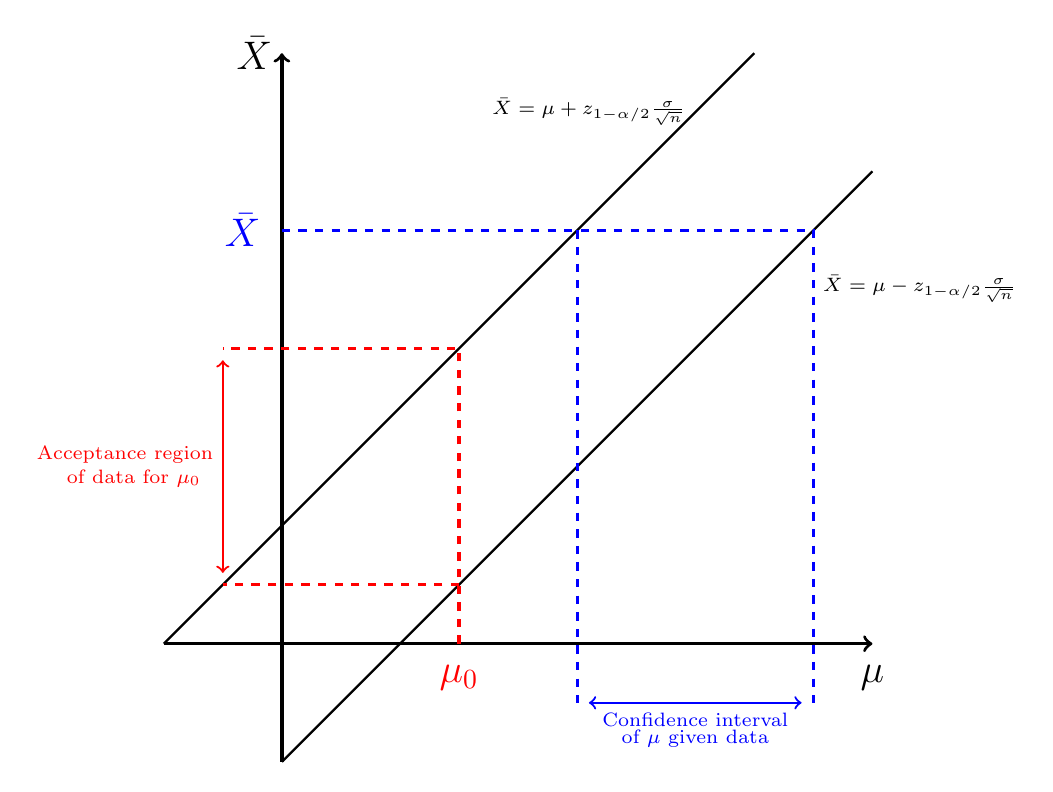
\begin{tikzpicture}[scale=0.75]
		\draw[->,very thick] (0,-2)--(0,10);
		\draw[->,very thick] (-2,0)--(10,0);
		
		\draw[thick] (-0,-2)--(10,8);
		\draw[thick] (-2,0)--(8,10);
		
		\node[left] at (0,10) {\Large$\bar{X}$};
		\node[below] at (10,-0.2) {\Large$\mu$};
		\node[left] at (-0.2,7) {\Large\textcolor{blue}{$\bar{X}$}};
		
		\node[below] at (3,-0.2) {\Large \textcolor{red}{$\mu_0$}};
		
		\draw[dashed, very thick, red] (3,0)--(3,5)--(-1,5);
		\draw[dashed, very thick, red] (3,1)--(-1,1);
		\draw[<->,thick,red] (-1,4.8)--(-1,1.2);
		\node[left] at (-1,3.2) {\scriptsize \textcolor{red}{Acceptance region}};
		\node[left] at (-1,2.8) {\scriptsize \textcolor{red}{of data for $\mu_0$}\;\;};
		
		\draw[dashed,very thick,blue] (0,7)--(9,7)--(9,-1);
		\draw[dashed,very thick,blue] (5,7)--(5,-1);
		\draw[<->,thick,blue] (5.2,-1)--(8.8,-1);
		\node[below] at (7,-1) {\scriptsize\textcolor{blue}{Confidence interval}};
		\node[below] at (7,-1.3) {\scriptsize\textcolor{blue}{of $\mu$ given data}};
		
		\node[right] at (9,6) {\scriptsize $\bar{X} = \mu - z_{1-\alpha/2} \frac{\sigma}{\sqrt{n}}$};
		\node[right] at (3.4,9) {\scriptsize $\bar{X} = \mu + z_{1-\alpha/2} \frac{\sigma}{\sqrt{n}}$};
	\end{tikzpicture}
	\caption{Confidence Intervals and Hypothesis Testing}
\end{figure}






















\end{document}